\chapter{Demostración y análisis del sistema}

En este capítulo se recorre la aplicación desde el punto de vista del usuario final y se analizan las visualizaciones principales, explicando qué muestra cada una y cómo interpretarla.

\section{Páginas implementadas}

A continuación se describen las vistas principales de la aplicación y su propósito.

\subsection{Página principal}
La página principal o ``home'' se ha buscado que sea muy sencilla, sólo se muestra el nombre dado a la plataforma, MIMIC-IV Analytics, junto a un pequeño subtítulo. 
\begin{figure}[H]
  \centering
  \fbox{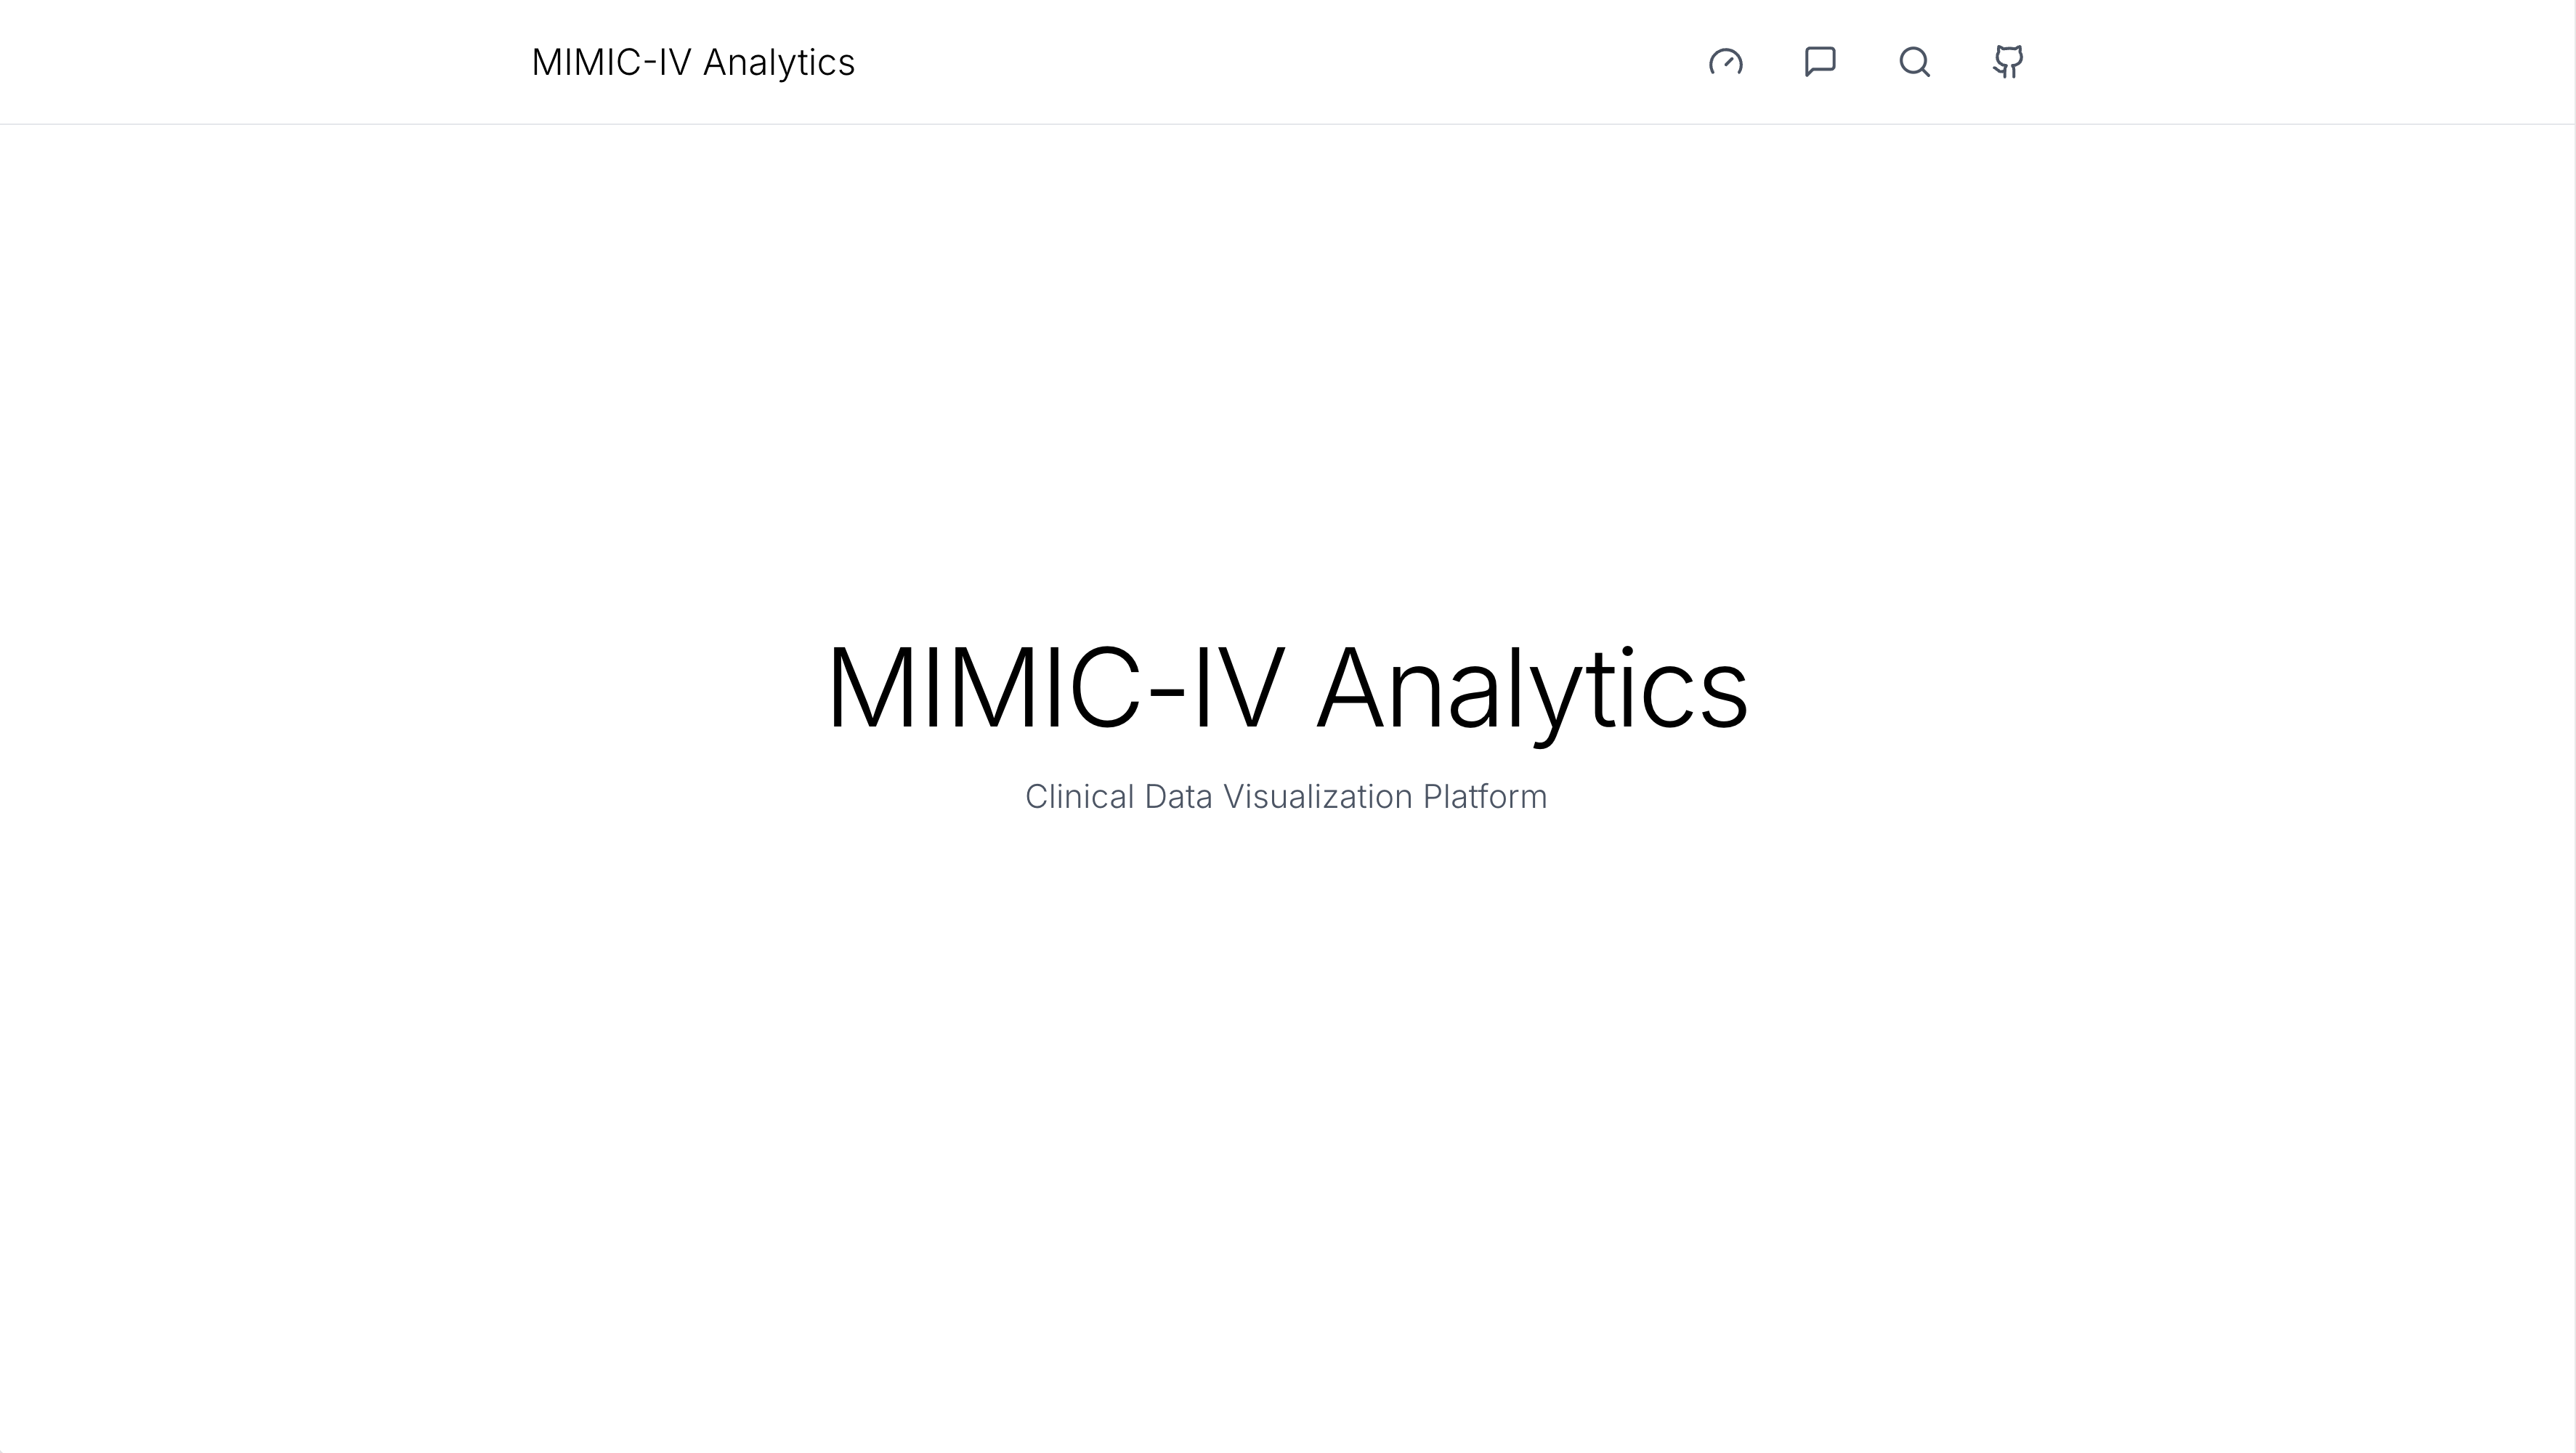
\includegraphics[width=1\textwidth]{imagenes/home.png}}
  \caption{Captura de pantalla de la página principal.}
  \label{fig:home}
\end{figure}

\subsection{Página del dashboard}
El objetivo de esta página es ofrecer al usuario una visión clara y accesible de las estadísticas más relevantes de la base de datos, seleccionadas por su importancia clínica. Para facilitar la interpretación y mejorar la experiencia de usuario, toda la información de MIMIC-IV se ha organizado en cinco grandes categorías: Demográficos y Admisiones, Cuidados Intensivos, Laboratorio y Medicamentos, Diagnósticos y Procedimientos, y Flujos Hospitalarios. En cada una de estas categorías se presentan tres indicadores estadísticos destacados, junto con enlaces a las visualizaciones asociadas. En total, se han implementado seis visualizaciones: dos para la categoría de Demográficos y Admisiones, y una para cada una de las categorías restantes.

En un entorno médico real e ideal, estos datos se actualizarían dinámicamente, permitiendo monitorizar de un vistazo los principales KPIs (Key Performance Indicators) y facilitando la toma de decisiones. Esta página sienta las bases para desarrollos futuros, en los que los profesionales sanitarios podrían filtrar los datos por periodos de tiempo, realizar comparativas o explorar tendencias, obteniendo así información relevante y actualizada sobre el estado del hospital. 
\begin{figure}[H]
  \centering
  \fbox{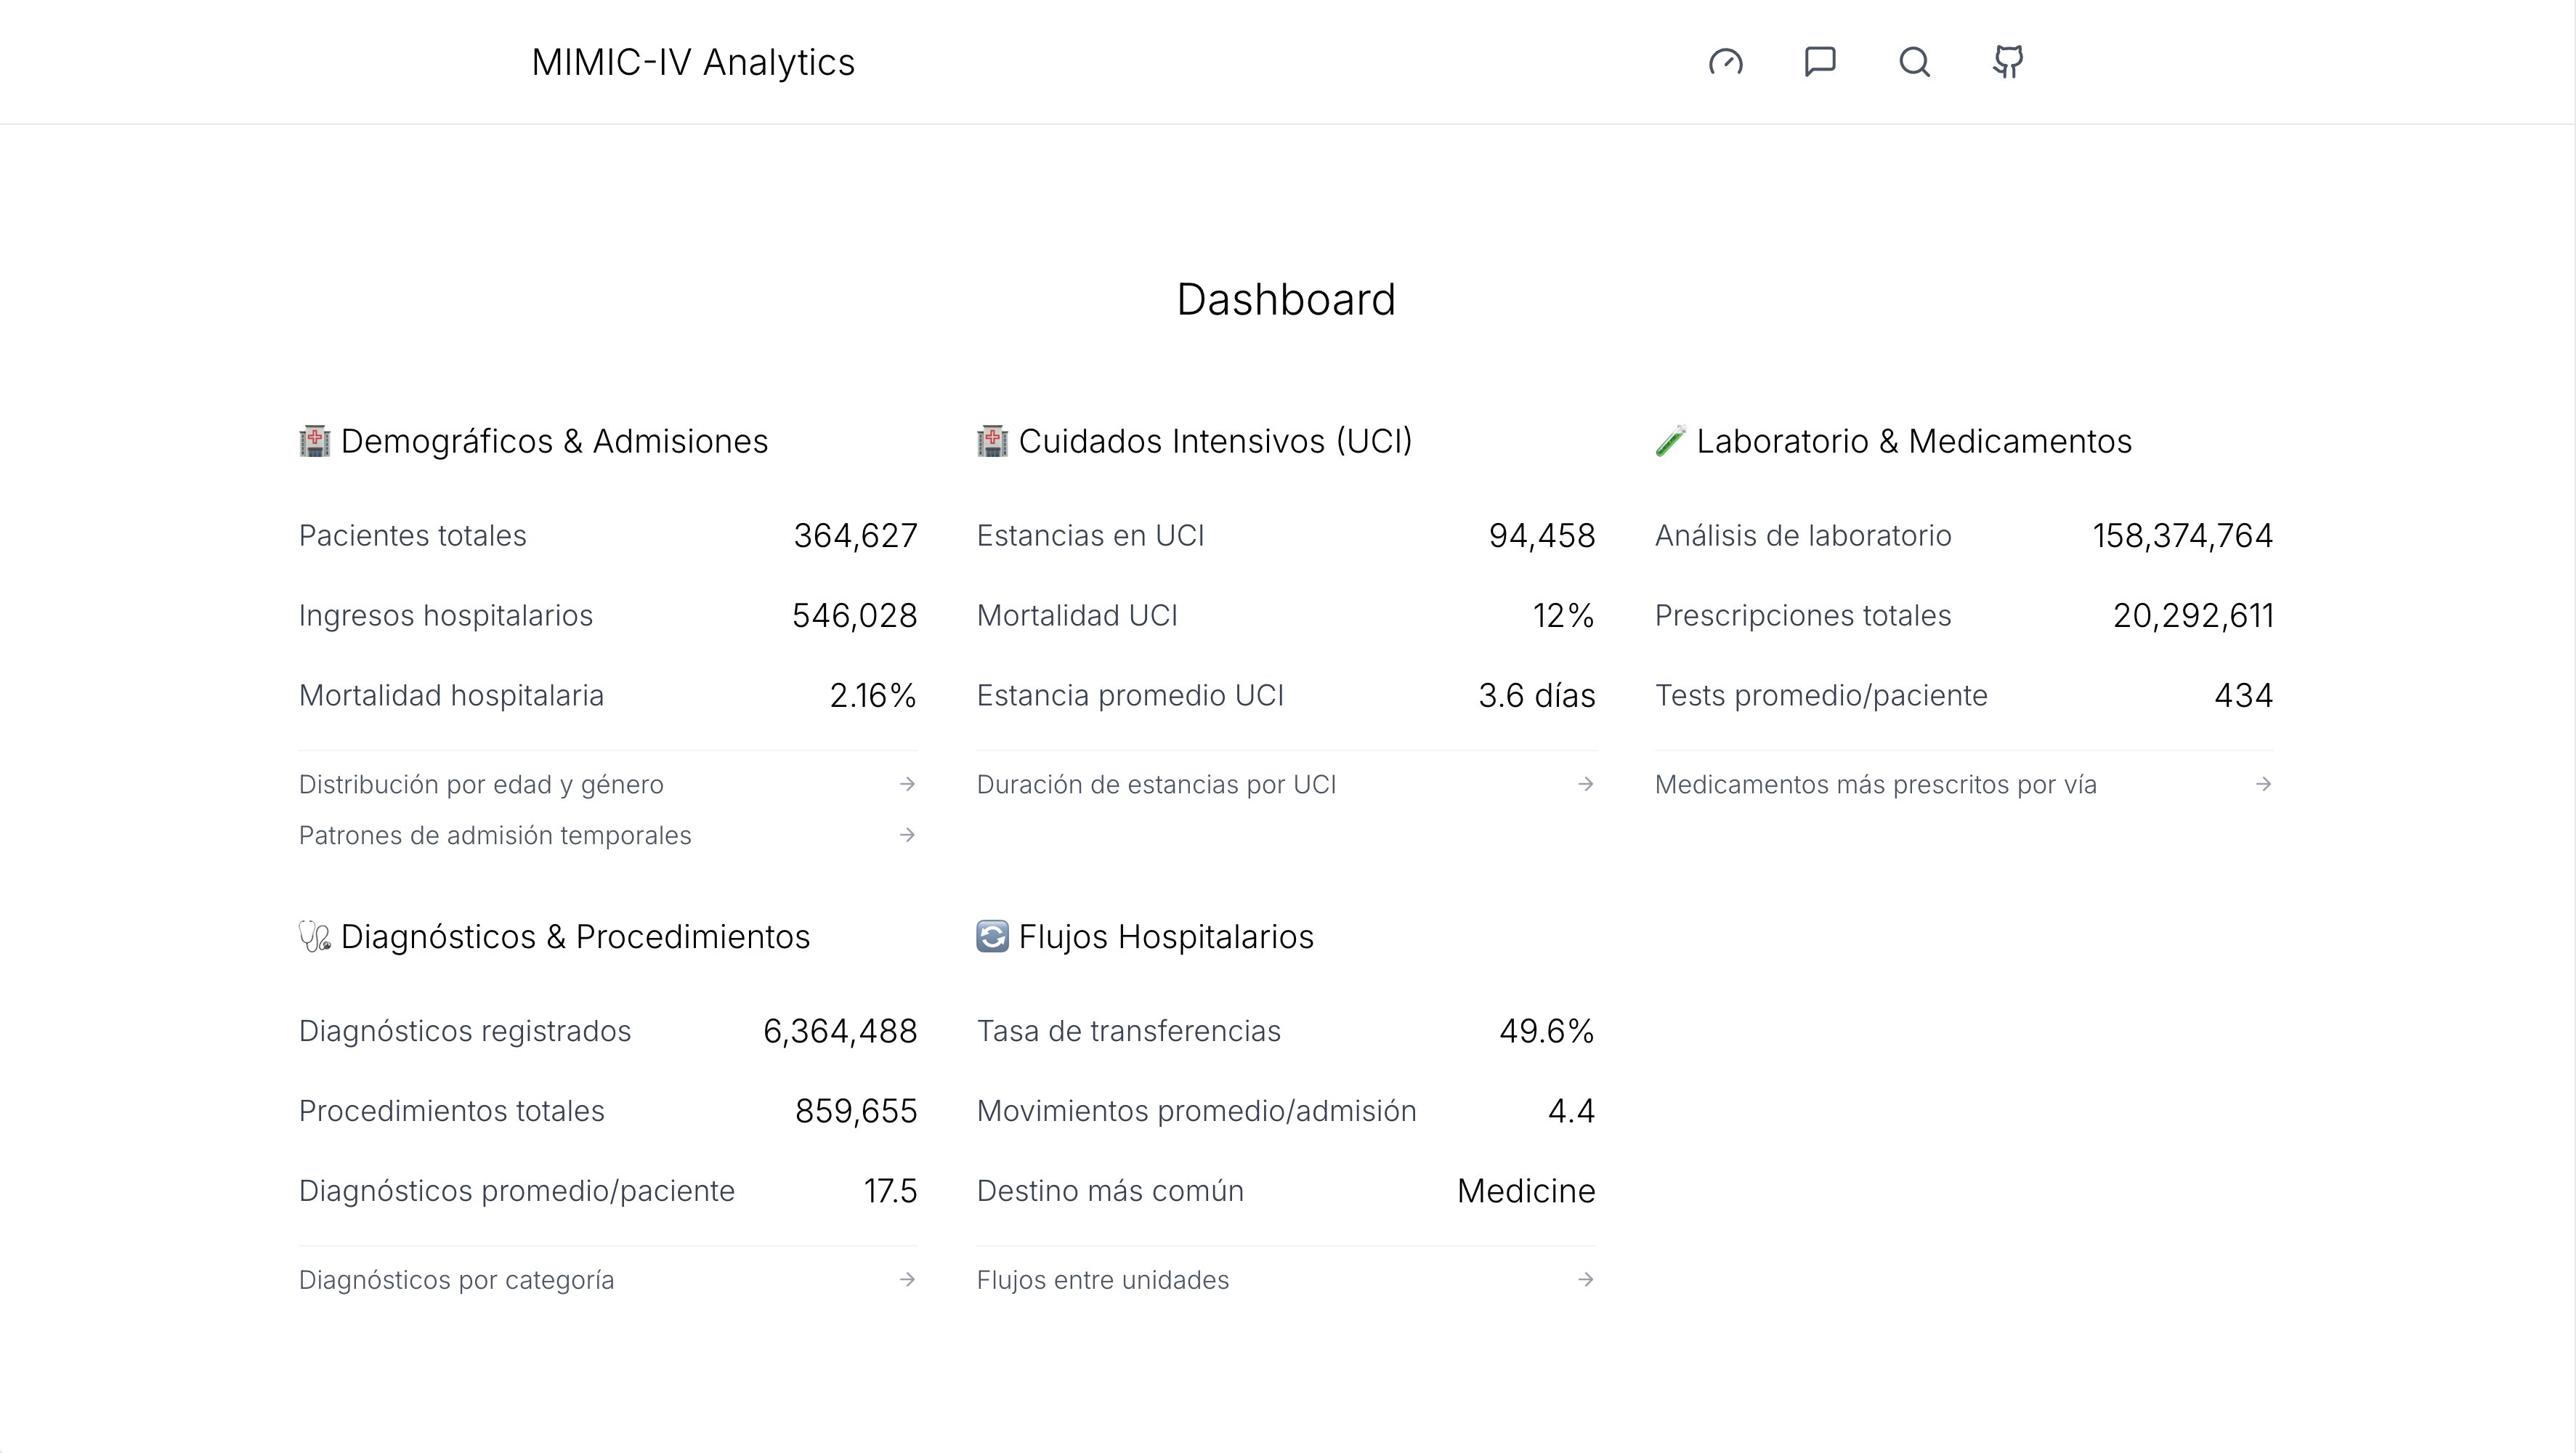
\includegraphics[width=1\textwidth]{imagenes/dash.png}}
  \caption{Captura de pantalla de la página del dashboard.}
  \label{fig:dash}
\end{figure}

\subsection{Página del chat}
Para la página del chat se sigue con la estética visual minimalista ya establecida, y se implementa la conexión con el backend, que ejecuta toda la lógica de comunicación entre el LLM, la base de datos gracias al protocolo MCP, y el frontend.
\begin{figure}[H]
  \centering
  \fbox{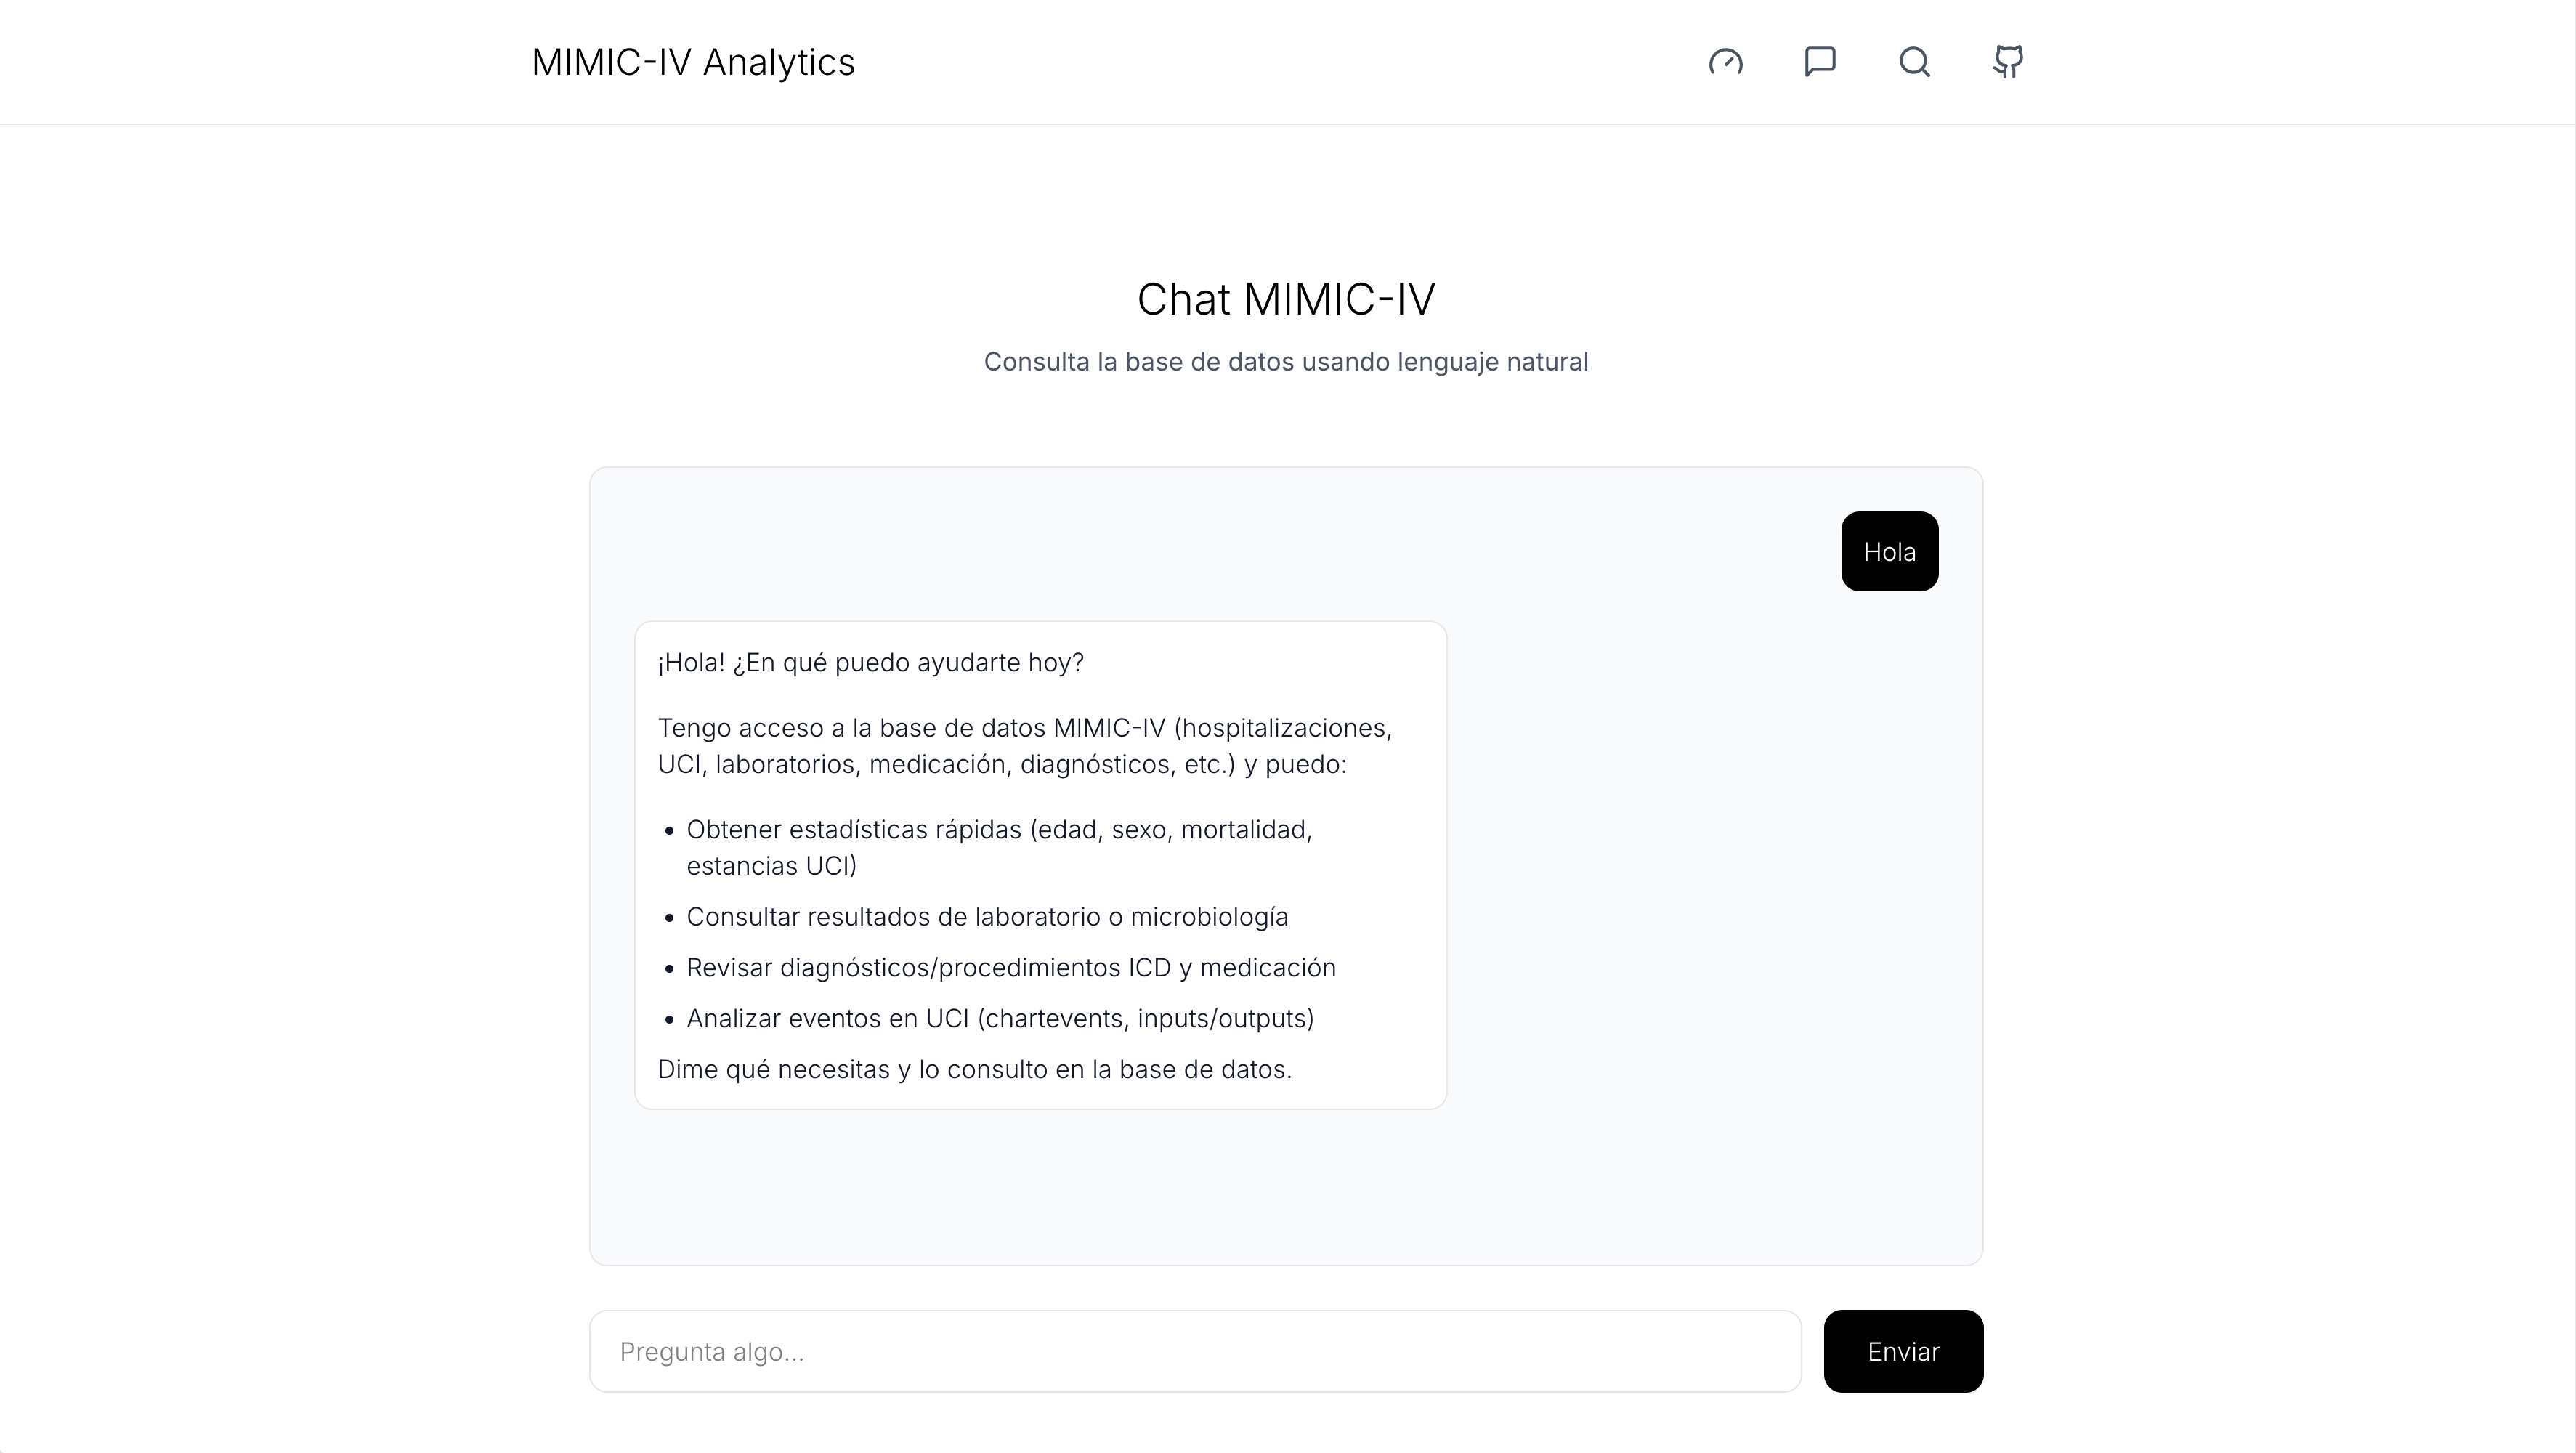
\includegraphics[width=1\textwidth]{imagenes/chat.png}}
  \caption{Captura de pantalla de la página del chat.}
  \label{fig:chat}
\end{figure}

\subsection{Página de búsqueda de pacientes}
Esta sencilla página nos permite comprobar la existencia de un paciente mediante su identificador único, mediante llamadas al endpoint del backend \texttt{/api/patients/\$\{id\}/exists}, y si es así (obtenemos status code 200 OK) entonces redirigimos a la página individual del paciente \texttt{/patient/\$\{id\}}. 
\begin{figure}[H]
  \centering
  \fbox{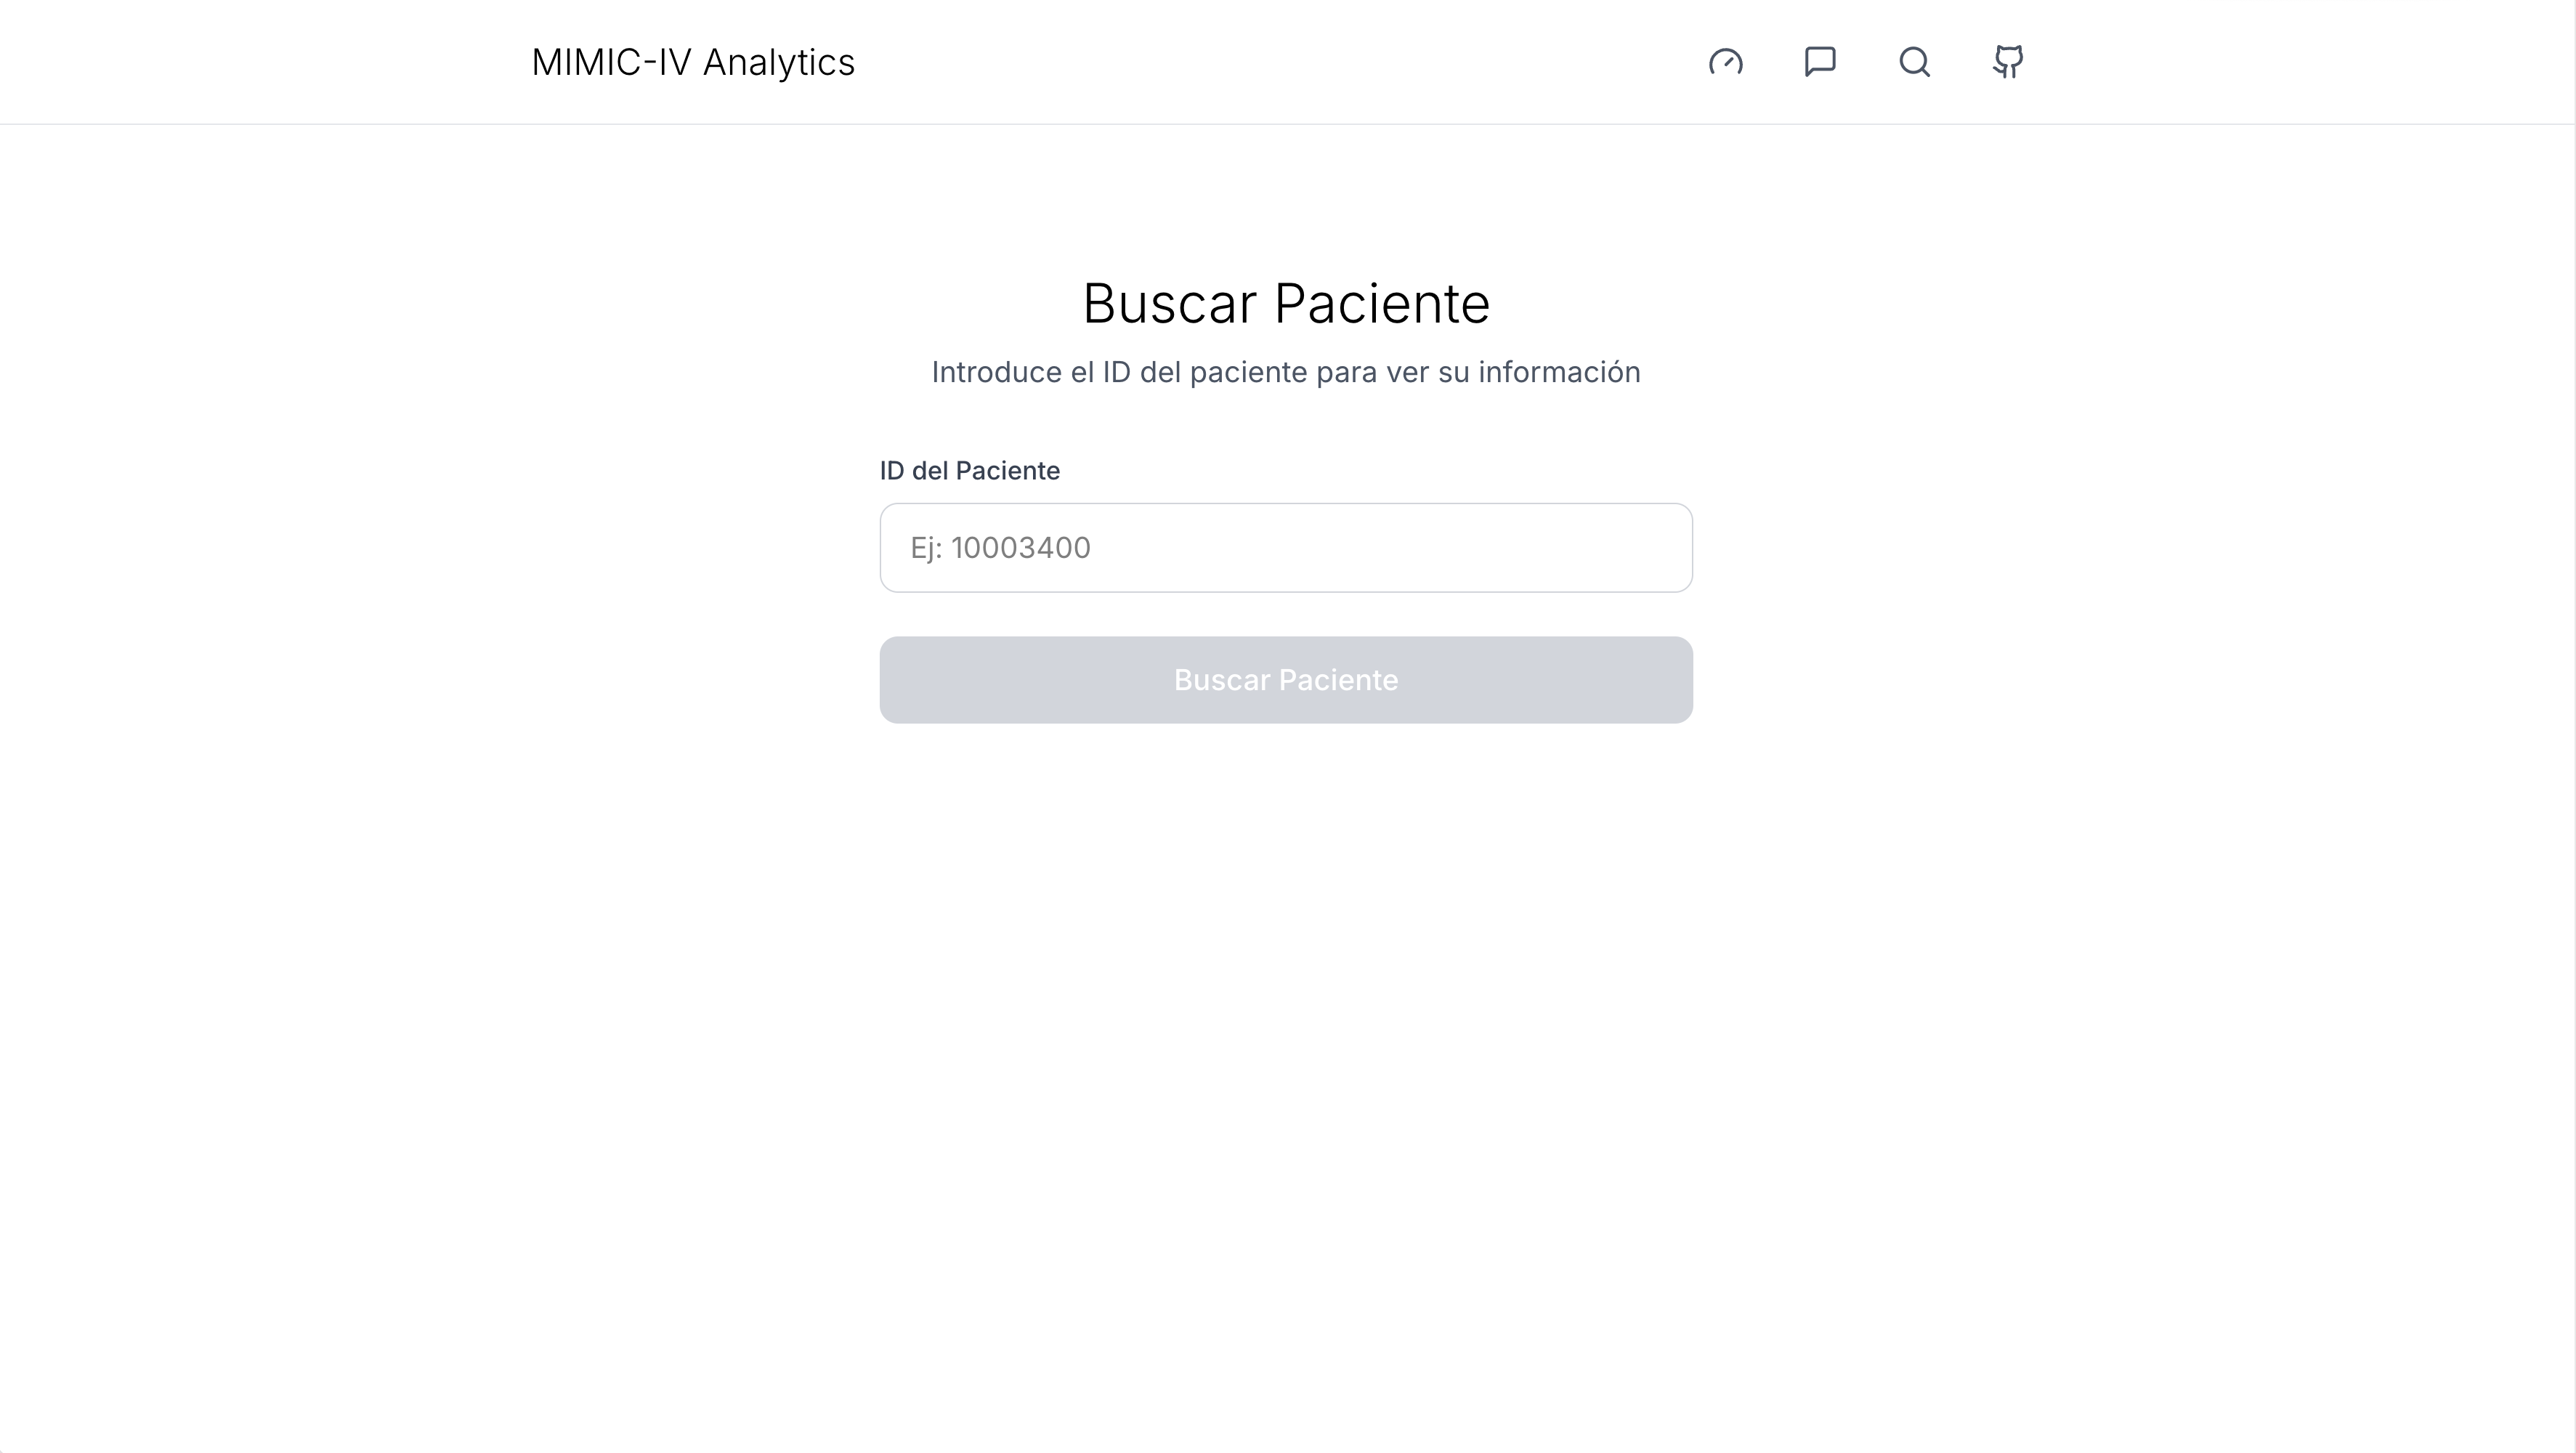
\includegraphics[width=1\textwidth]{imagenes/search.png}}
  \caption{Captura de pantalla de la página de búsqueda de pacientes.}
  \label{fig:search}
\end{figure}

\subsection{Página del paciente individual}
Al aterrizar en una de estas páginas, lo que hacemos es obtener el ID del paciente (\texttt{subject\_id}) de la URL, y lo envíamos al backend, a la ruta \texttt{/api/patients/\$\{id\}}. Este nos devuelve absolutamente toda la información relacionada con el paciente que necesitamos, por lo que puede tardar varios segundos en responder. Una vez con los datos, los mostramos de forma estructurada y visualmente agradable. A continuación se explican las tres secciones distintas en las que se ha organizado la información, las cuales han sido implementadas como componentes distintos que reciben los datos que necesitan de la página padre.

En primer lugar encontramos una sección con la información demográfica básica del paciente: género, edad, idioma, raza, etc. Implementado en el componente React \texttt{PatientBasicInfo}.

En segundo lugar, una sección en la que se muestra un resumen del paciente realizada con Inteligencia Artificial. El funcionamiento es el siguiente: una vez se reciben todos los datos del paciente y se carga la página, automáticamente el componente \texttt{PatientAISummary} llama a otro endpoint del backend \texttt{/api/summary/patient} y le envía todos los datos del paciente, para que se llame al LLM y se obtenga el resumen del historial. De esta forma, enviando los datos directamente y no el ID del paciente, nos ahorramos el tiempo de espera de volver a agregar toda información.

En tercer lugar tenemos el grueso de la información, en el componente \texttt{PatientAdmissions}. En el mediante desplegables, vemos un listado de todos los ingresos que ha tenido el paciente, junto a algunas estadísticas rápidas para ver a simple vista: número de días de duración de la hospitalización, número de diagnósticos asociados a la estancia, número de procedimientos, y número de tests de laboratorio. 

Al hacer click en el desplegable, podemos ver más información del ingreso, como las fechas exactas de entrada y salida, el tipo del seguro del paciente, a dónde se trasfirió despues, etc. Además, de nuevo, a forma de desplegables, podemos ver la información detallada de los diagnósticos, procedimientos, y tests de laboratorio.

En cuanto a los últimos, se ha implementado poder filtrar los tests según su categoría (Blood Gas, Hematology, Chemistry...) o bien verlos todos a la vez. De nuevo, se muestra el listado de los tests como un listado de elementos desplegables, búscando la limpieza visual al encapsular la información y visualizar sólo los datos que se quieren ver. Cuando se hace click en uno de los tests, si éste tiene dos o más ocurrencias, se mostrará una gráfica con la evolución temporal para dicha métrica. 
\begin{figure}[H]
  \centering
  \fbox{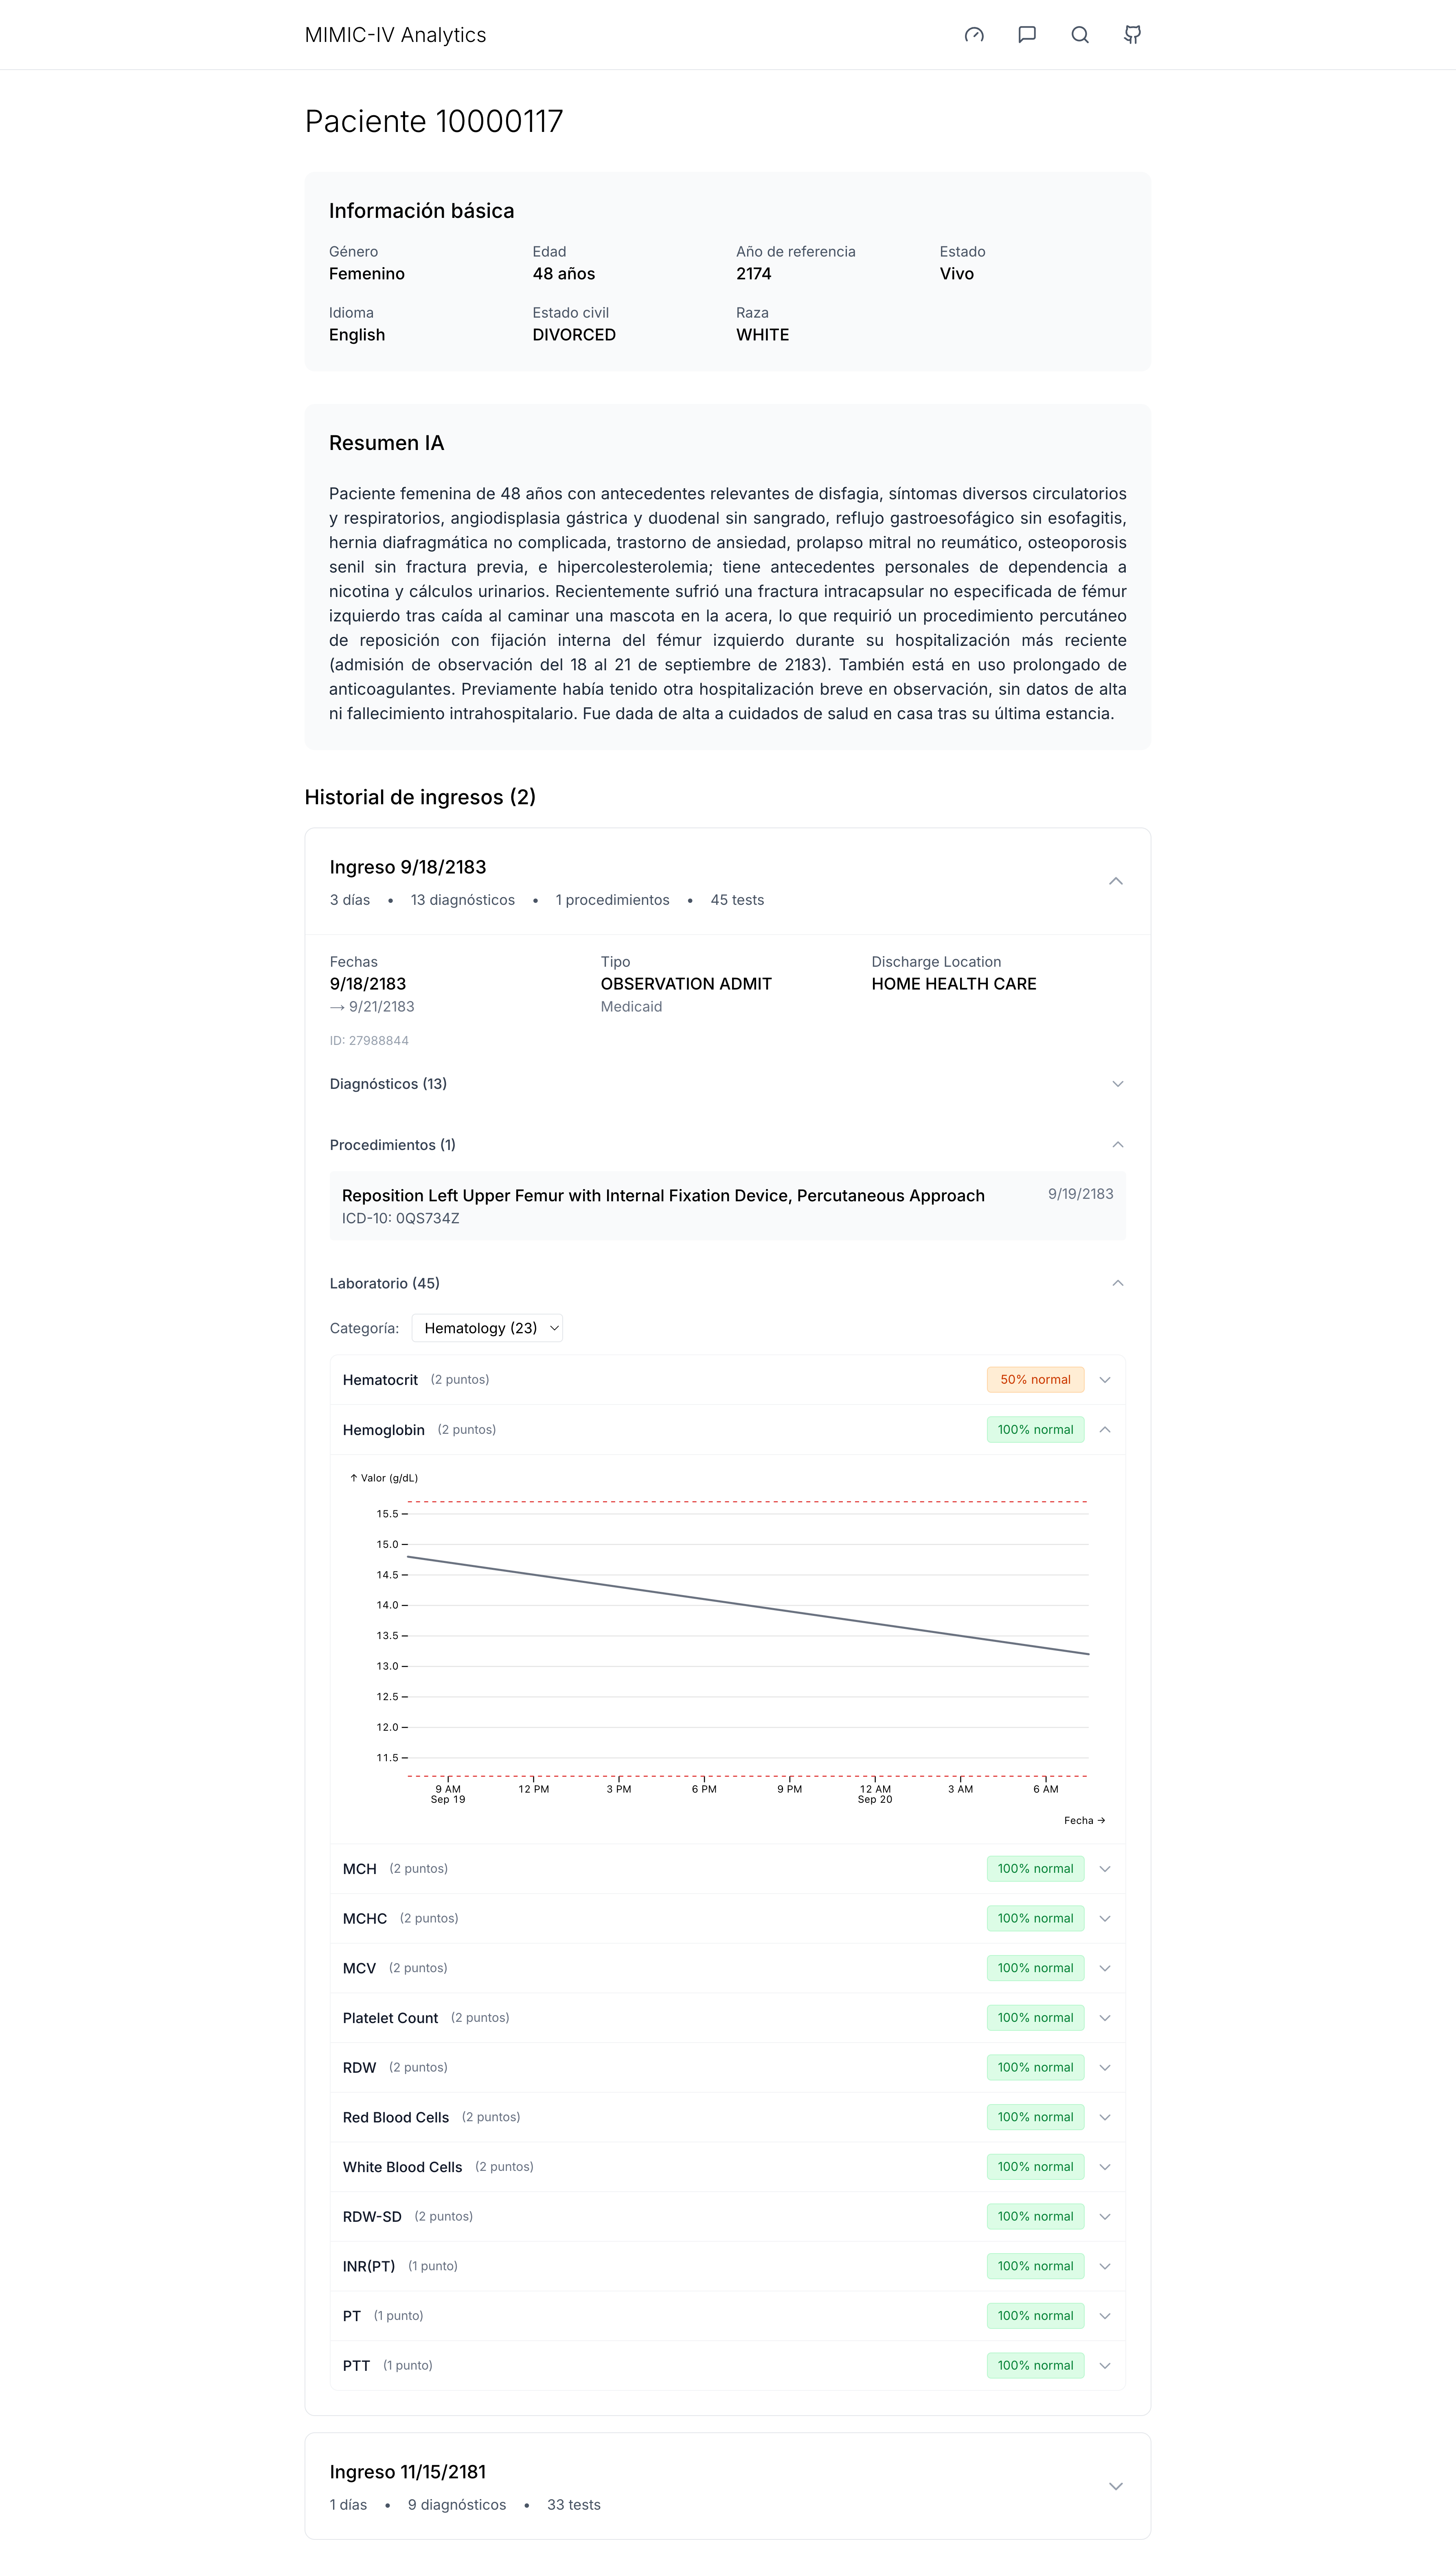
\includegraphics[width=0.9\textwidth]{imagenes/patient1.png}}
  \caption{Captura de pantalla de la página del paciente.}
  \label{fig:patient}
\end{figure}

\section{Visualizaciones y lectura}

En esta sección se describen las visualizaciones de datos que se han implementado.

\subsection{Distribución por edad y género}
Ahora vamos a pasar a las visualizaciones de datos que se han implementado. El primer gráfico, realizado utilizando Observable Plot, es un Population Pyramid \cite{populationPyramid} de la distribución por edad y género, con dos variantes, una por rangos de edad, y la otra por edad específica.
\begin{figure}[H]
  \centering
  \fbox{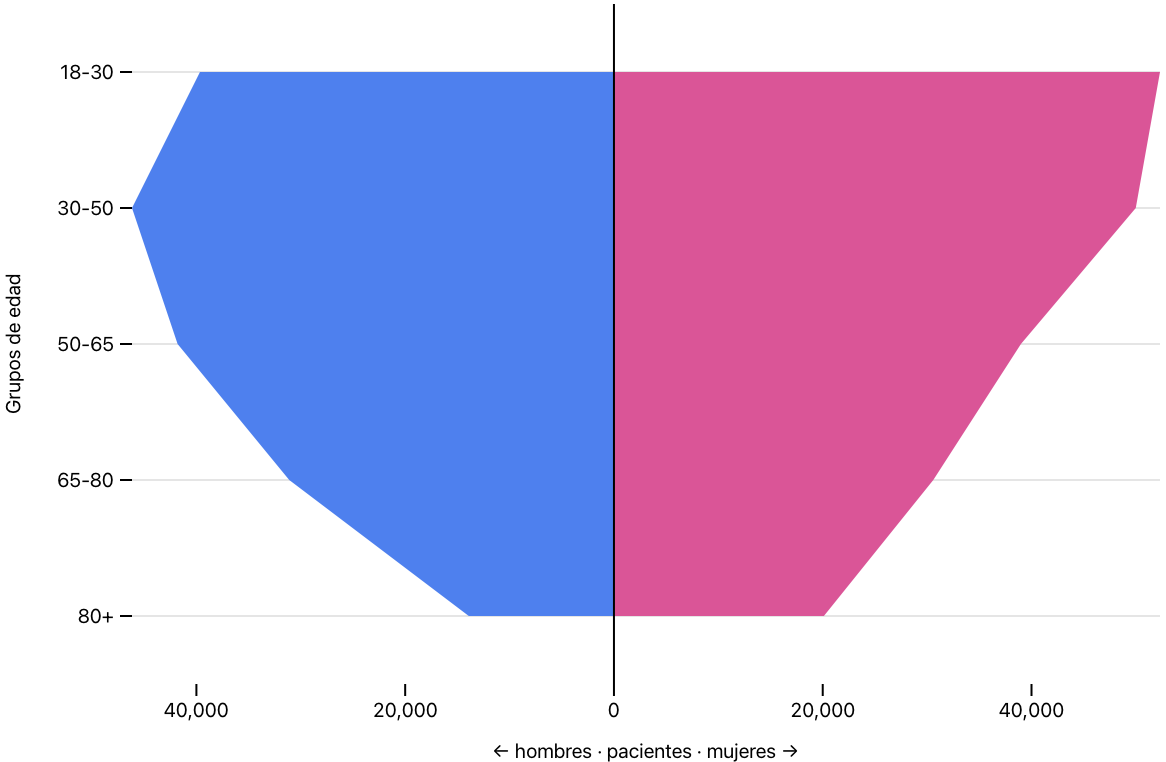
\includegraphics[width=0.65\textwidth]{imagenes/chart2.png}}
  \caption{Distribución por edad y género (rangos de edad)}
  \label{fig:chart2}
\end{figure}
\begin{figure}[H]
  \centering
  \fbox{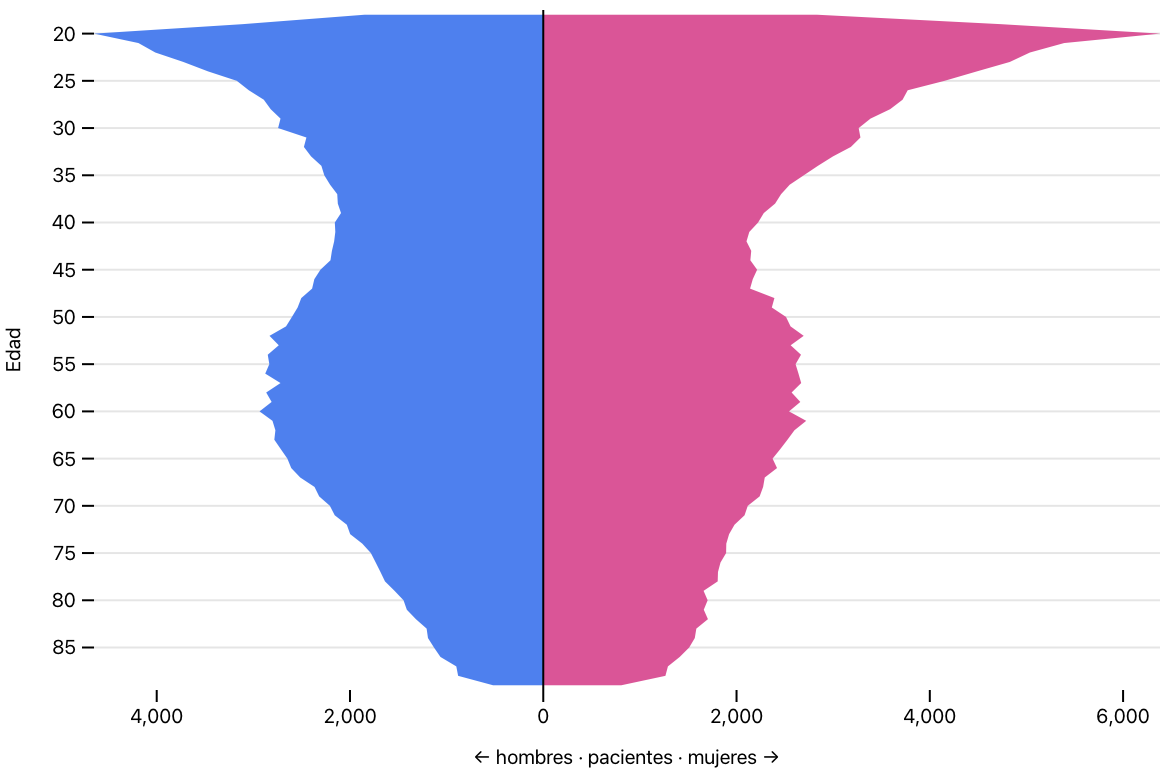
\includegraphics[width=0.65\textwidth]{imagenes/chart3.png}}
  \caption{Distribución por edad y género}
  \label{fig:chart3}
\end{figure}

\subsection{Heatmap de ingresos}
El segundo gráfico, también desarrollado con Observable Plot, consiste en un heatmap\cite{heatmap} que representa la cantidad de ingresos hospitalarios en función de la hora y la fecha, ofreciendo dos variantes. La primera muestra los ingresos distribuidos por horas y días de la semana, lo que permite identificar los periodos de mayor y menor actividad en el hospital. Durante el desarrollo se detectó una concentración anómala de ingresos a las 00:00:00, de lo que se dedujo que se trataban de registros en los que la hora real de ingreso no estaba disponible; por ello, se filtraron estos casos del gráfico principal, aunque se dejó la opción de visualizarlos mediante un botón para que el usuario pueda acceder siempre a la información completa.

La segunda variante del heatmap representa los ingresos por mes y día del mes. Aquí, el día 29 de febrero presentaba un número de ingresos significativamente inferior, lo que distorsionaba la escala de colores y oscurecía el resto de los datos. Para evitar este efecto, se optó por excluir ese día del gráfico principal y mostrar su valor de forma separada, garantizando así una visualización más precisa y homogénea del resto de los datos.
\begin{figure}[H]
  \centering
  \fbox{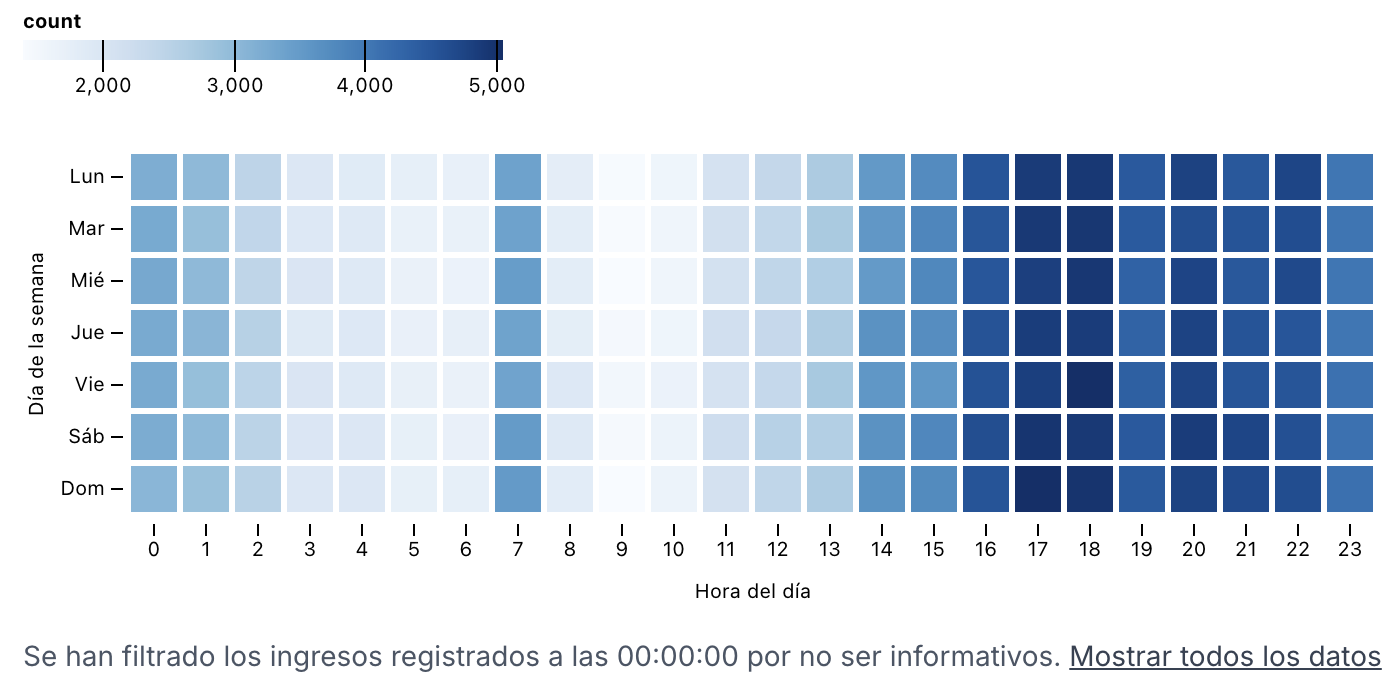
\includegraphics[width=0.8\textwidth]{imagenes/chart-heat-1.png}}
  \caption{Heatmap de ingresos por hora y día de la semana.}
  \label{fig:chart-heat-1}
\end{figure}
\begin{figure}[H]
  \centering
  \fbox{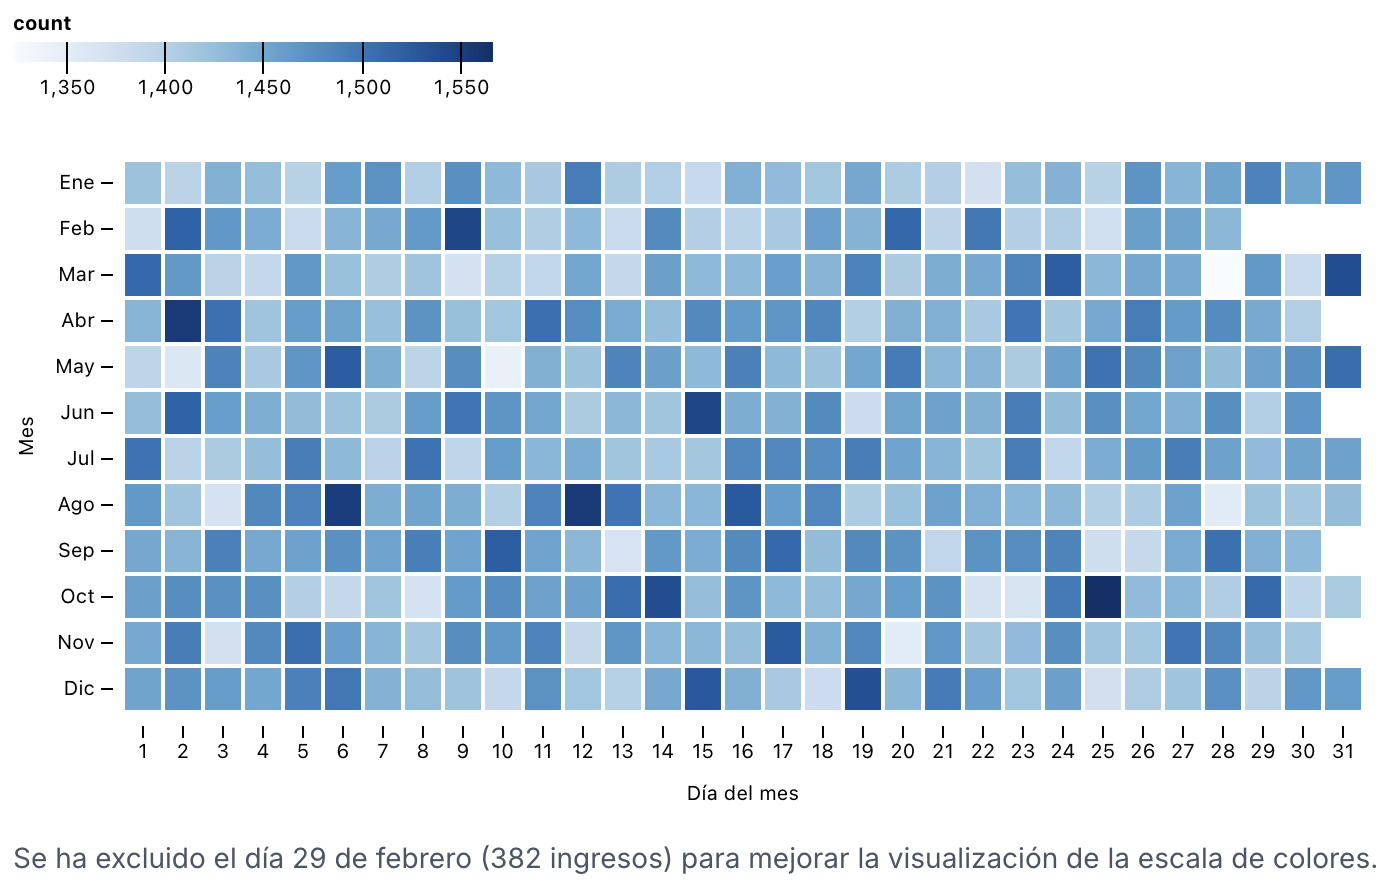
\includegraphics[width=0.8\textwidth]{imagenes/chart-heat-2.png}}
  \caption{Heatmap de ingresos por mes y día del mes.}
  \label{fig:chart-heat-2}
\end{figure}

\subsection{Estancia promedio por unidad UCI}
Este gráfico, un Horizontal Bar Chart \cite{hbarchart} de Observable Plot, muestra cual es el  número de días promedio de estancia para cada unidad UCI. Se ha implementado un input para modificar el umbral mínimo de estancias, ya que hay unidades con muy pocas estancias que pueden no ser informativas. Un ejemplo es la unidad \texttt{Neurology}, que sólo tiene una estancia, y es de 28 días, muy por encima del resto. 
\begin{figure}[H]
  \centering
  \fbox{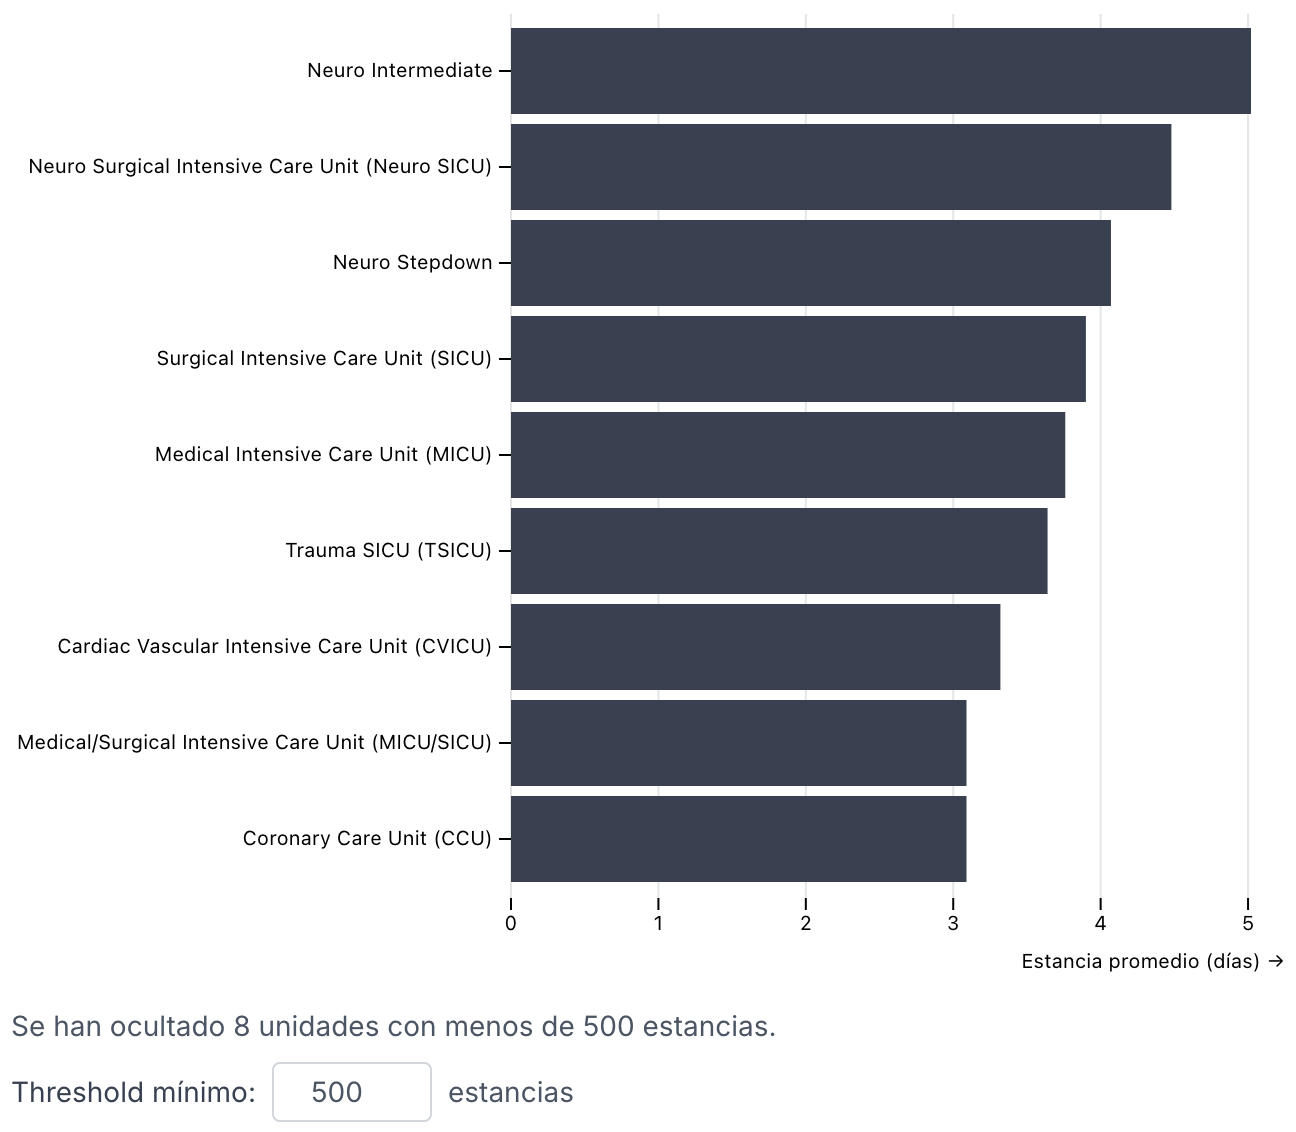
\includegraphics[width=0.75\textwidth]{imagenes/chart-icu.png}}
  \caption{Estancia promedio por unidad UCI}
  \label{fig:chart-icu}
\end{figure}

\subsection{Medicamentos más prescritos por vía}
Esta visualización es más compleja que las anteriores, por lo que se hace uso de la librería D3. Se trata de un gráfico Sunburst interactivo \cite{sunburst}, que permite hacer zoom para moverse por la información. Se muestran los medicamentos más prescritos por vía de administración. Para este gráfico, debido a la enorme cantidad de documentos (más de 20 millones) en la colección donde se aloja esta información \texttt{hosp\_prescriptions}, en lugar de obtener los datos en cada llamada al endpoint del backend, se ha realizado una colección nueva mediante un script Python, que contiene los datos ya pre-agregados, consiguiendo así obtener los datos mucho más rápido. También se implementan unos filtros de umbral mínimo y máximo para facilitar la visualización.
\begin{figure}[H]
  \centering
  \fbox{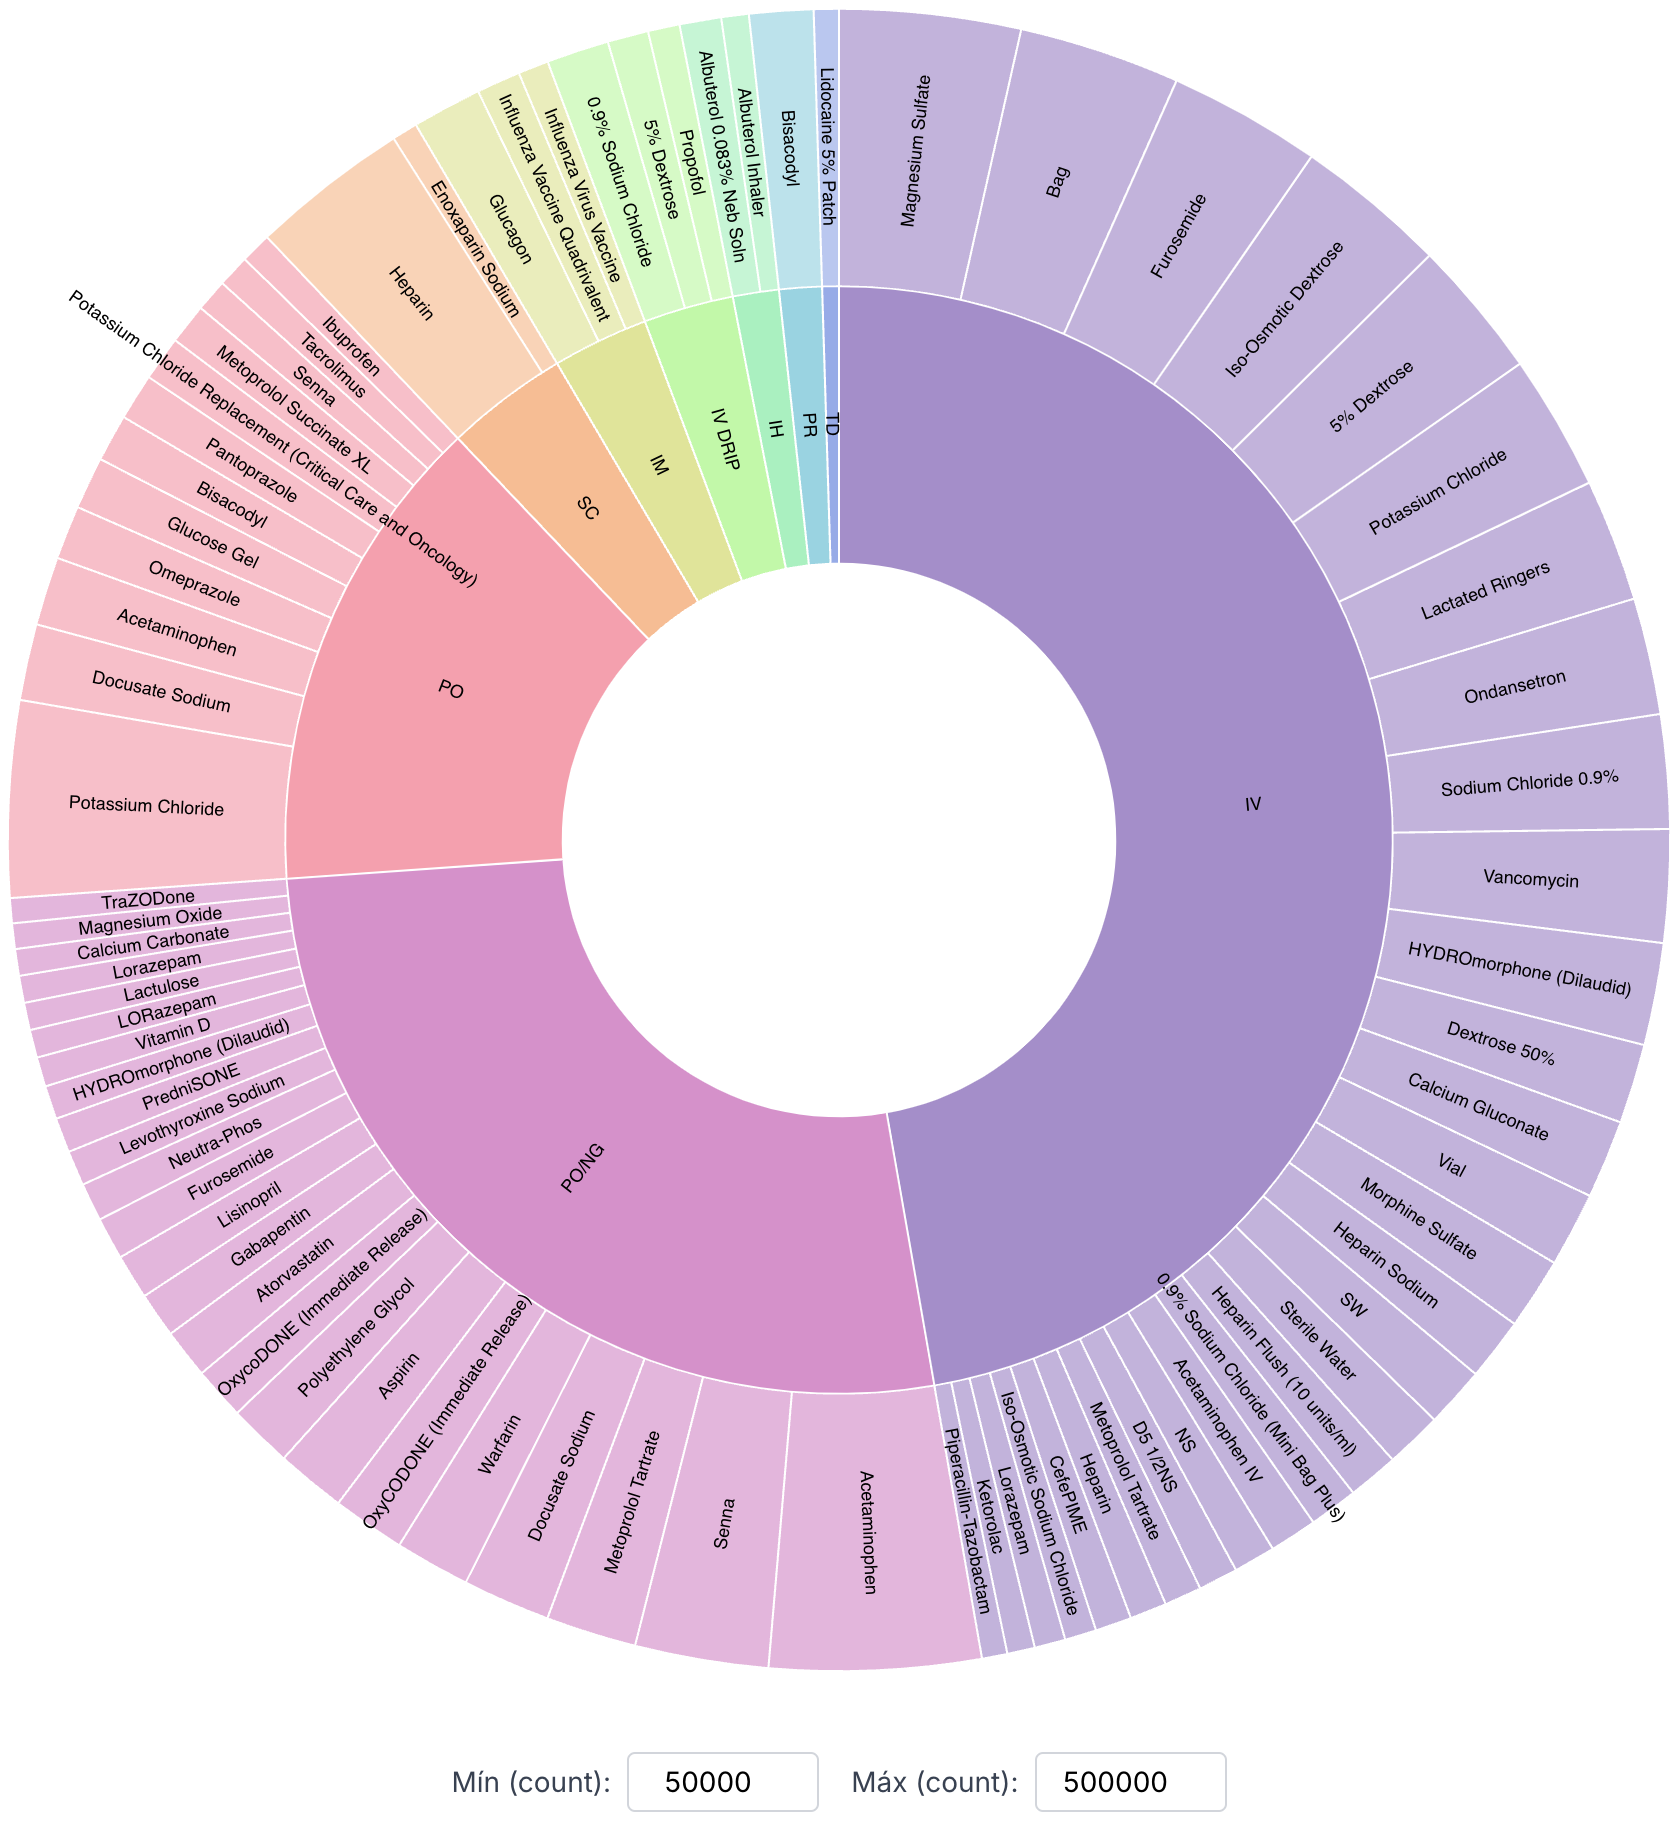
\includegraphics[width=0.85\textwidth]{imagenes/chart-sunburst.png}}
  \caption{Medicamentos más prescritos por vía}
  \label{fig:chart-sunburst}
\end{figure}

\subsection{Diagnósticos por categoría}
En este caso se presenta de nuevo un gráfico interactivo realizado con D3, denominado Icicle \cite{icicle}. El gráfico muestra todos los diagnósticos, con la opción de aplicar un filtro por umbral mínimo, y están organizados jerárquicamente según la tabla \texttt{icd\_equivalencias}, mencionada previamente. Esto permite visualizar no solo los diagnósticos más frecuentes, sino también las categorías superiores que los agrupan, haciendo zoom para ver la información detallada cuando se necesite. 

Para esta visualización también se necesitó implementar un script que realiza las agregaciones necesarias y las almacena en una colección de MongoDB nueva, debido a la imposibilidad de agregar todos los datos en cada petición, el tiempo de espera era demasiado alto.
\begin{figure}[H]
  \centering
  \fbox{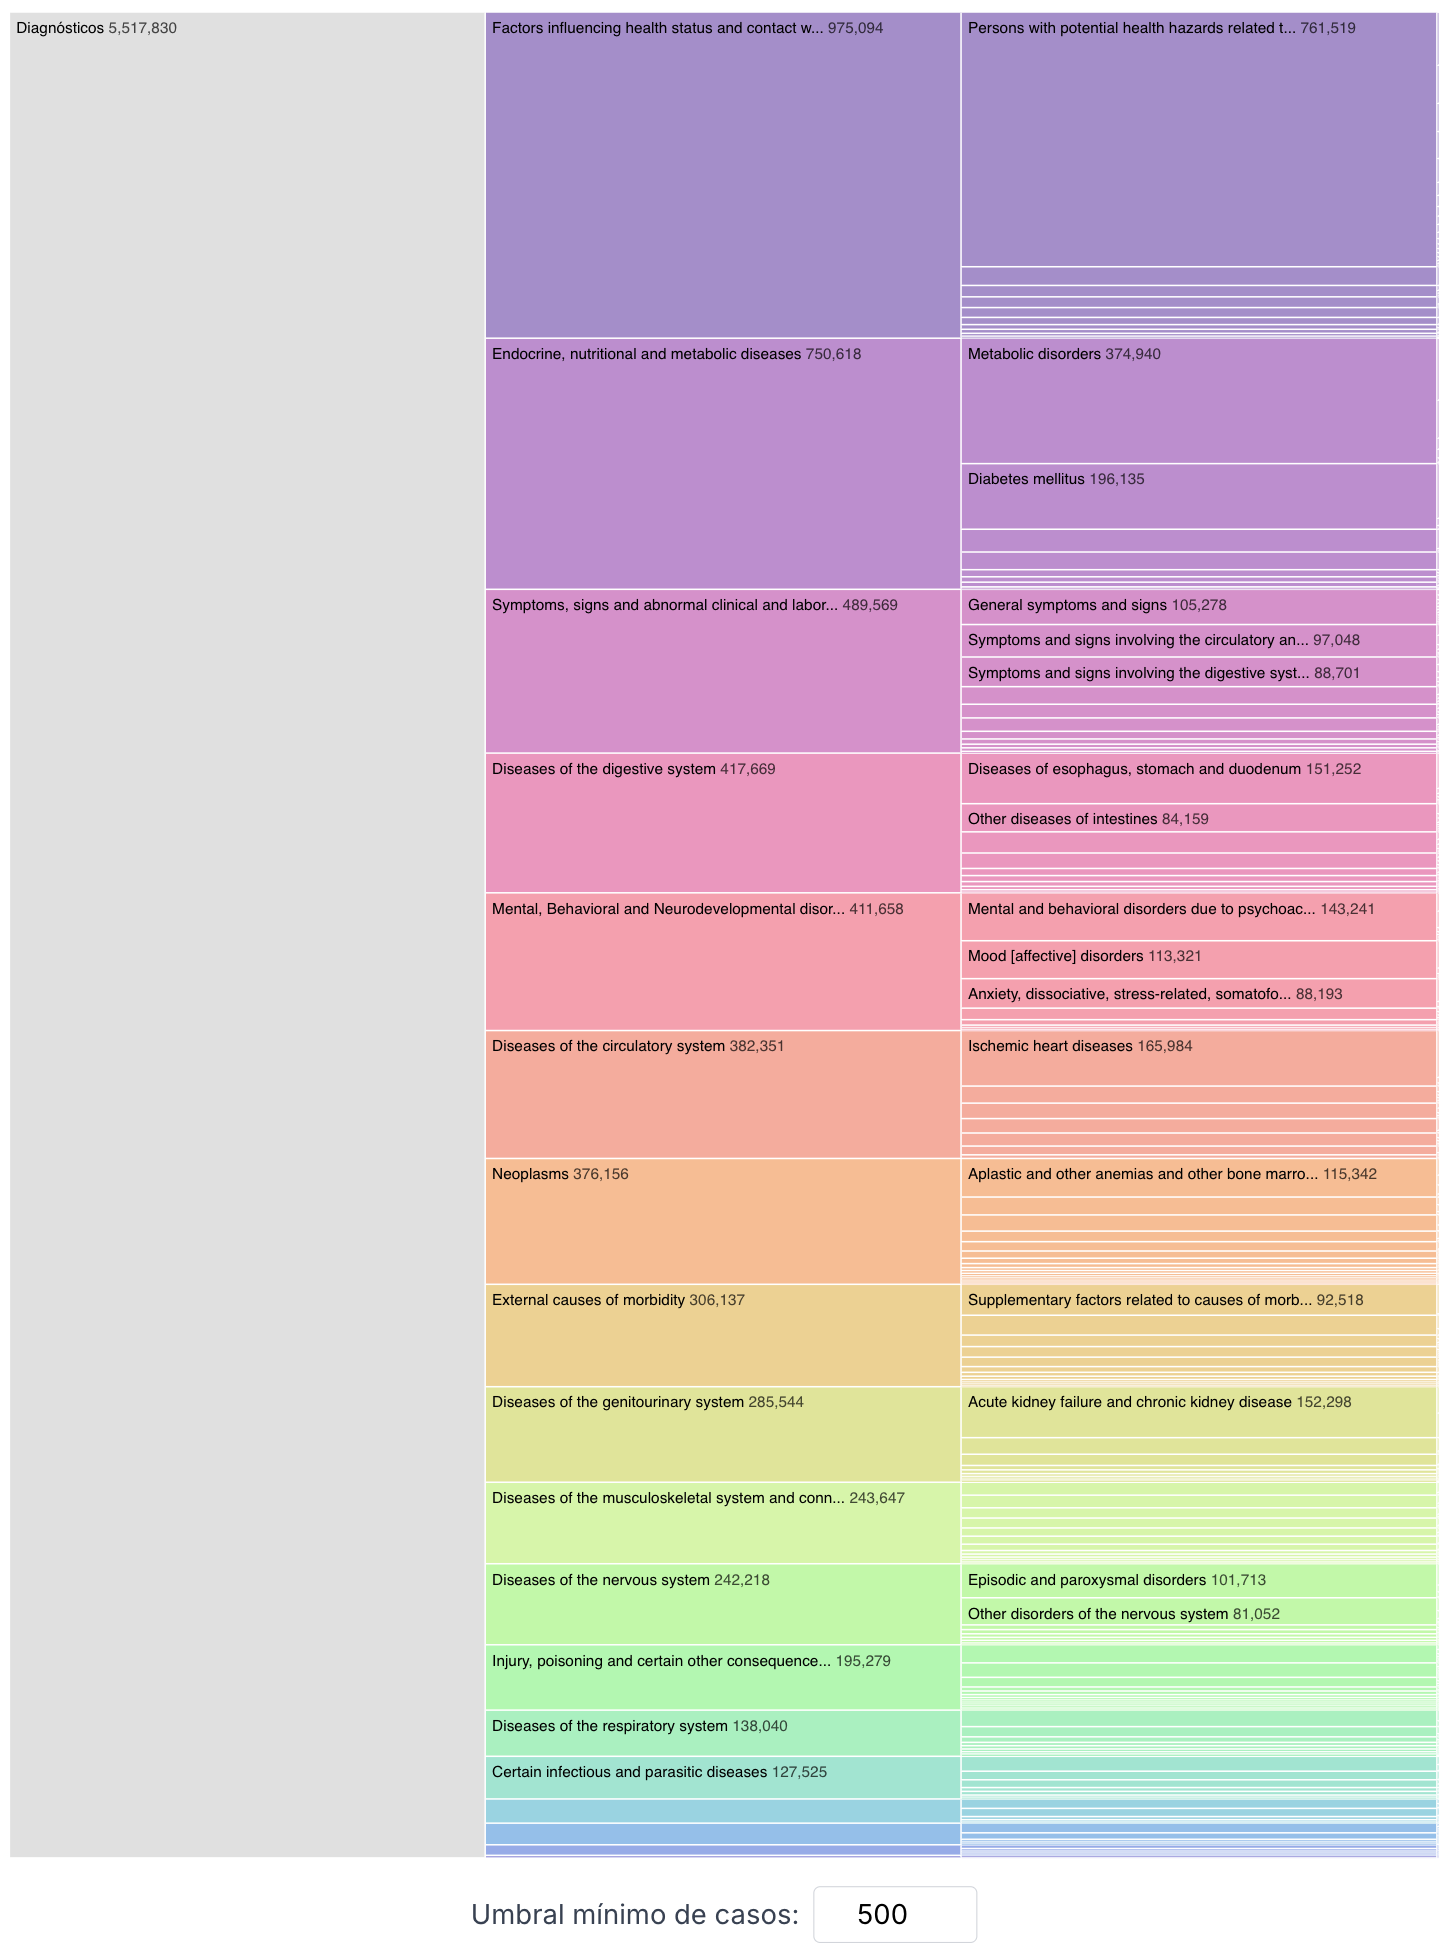
\includegraphics[width=0.88\textwidth]{imagenes/chart-diag.png}}
  \caption{Diagnósticos por categoría}
  \label{fig:chart-diag}
\end{figure}

\subsection{Flujos hospitalarios}
Este gráfico, al igual que los dos anteriores, utiliza D3 y en este caso, se trata de un Directed Chord Diagram \cite{chord}. Para su implementación, se crea una nueva colección con los datos pre-agregados. El gráfico representa la información de \texttt{hosp\_transfers}, mostrando la cantidad de transferencias hospitalarias entre unidades. Al pasar el cursor sobre cada conexión, se ven la unidad de origen, la de destino, y el recuento de transferencias de ese tipo.
\begin{figure}[H]
  \centering
  \fbox{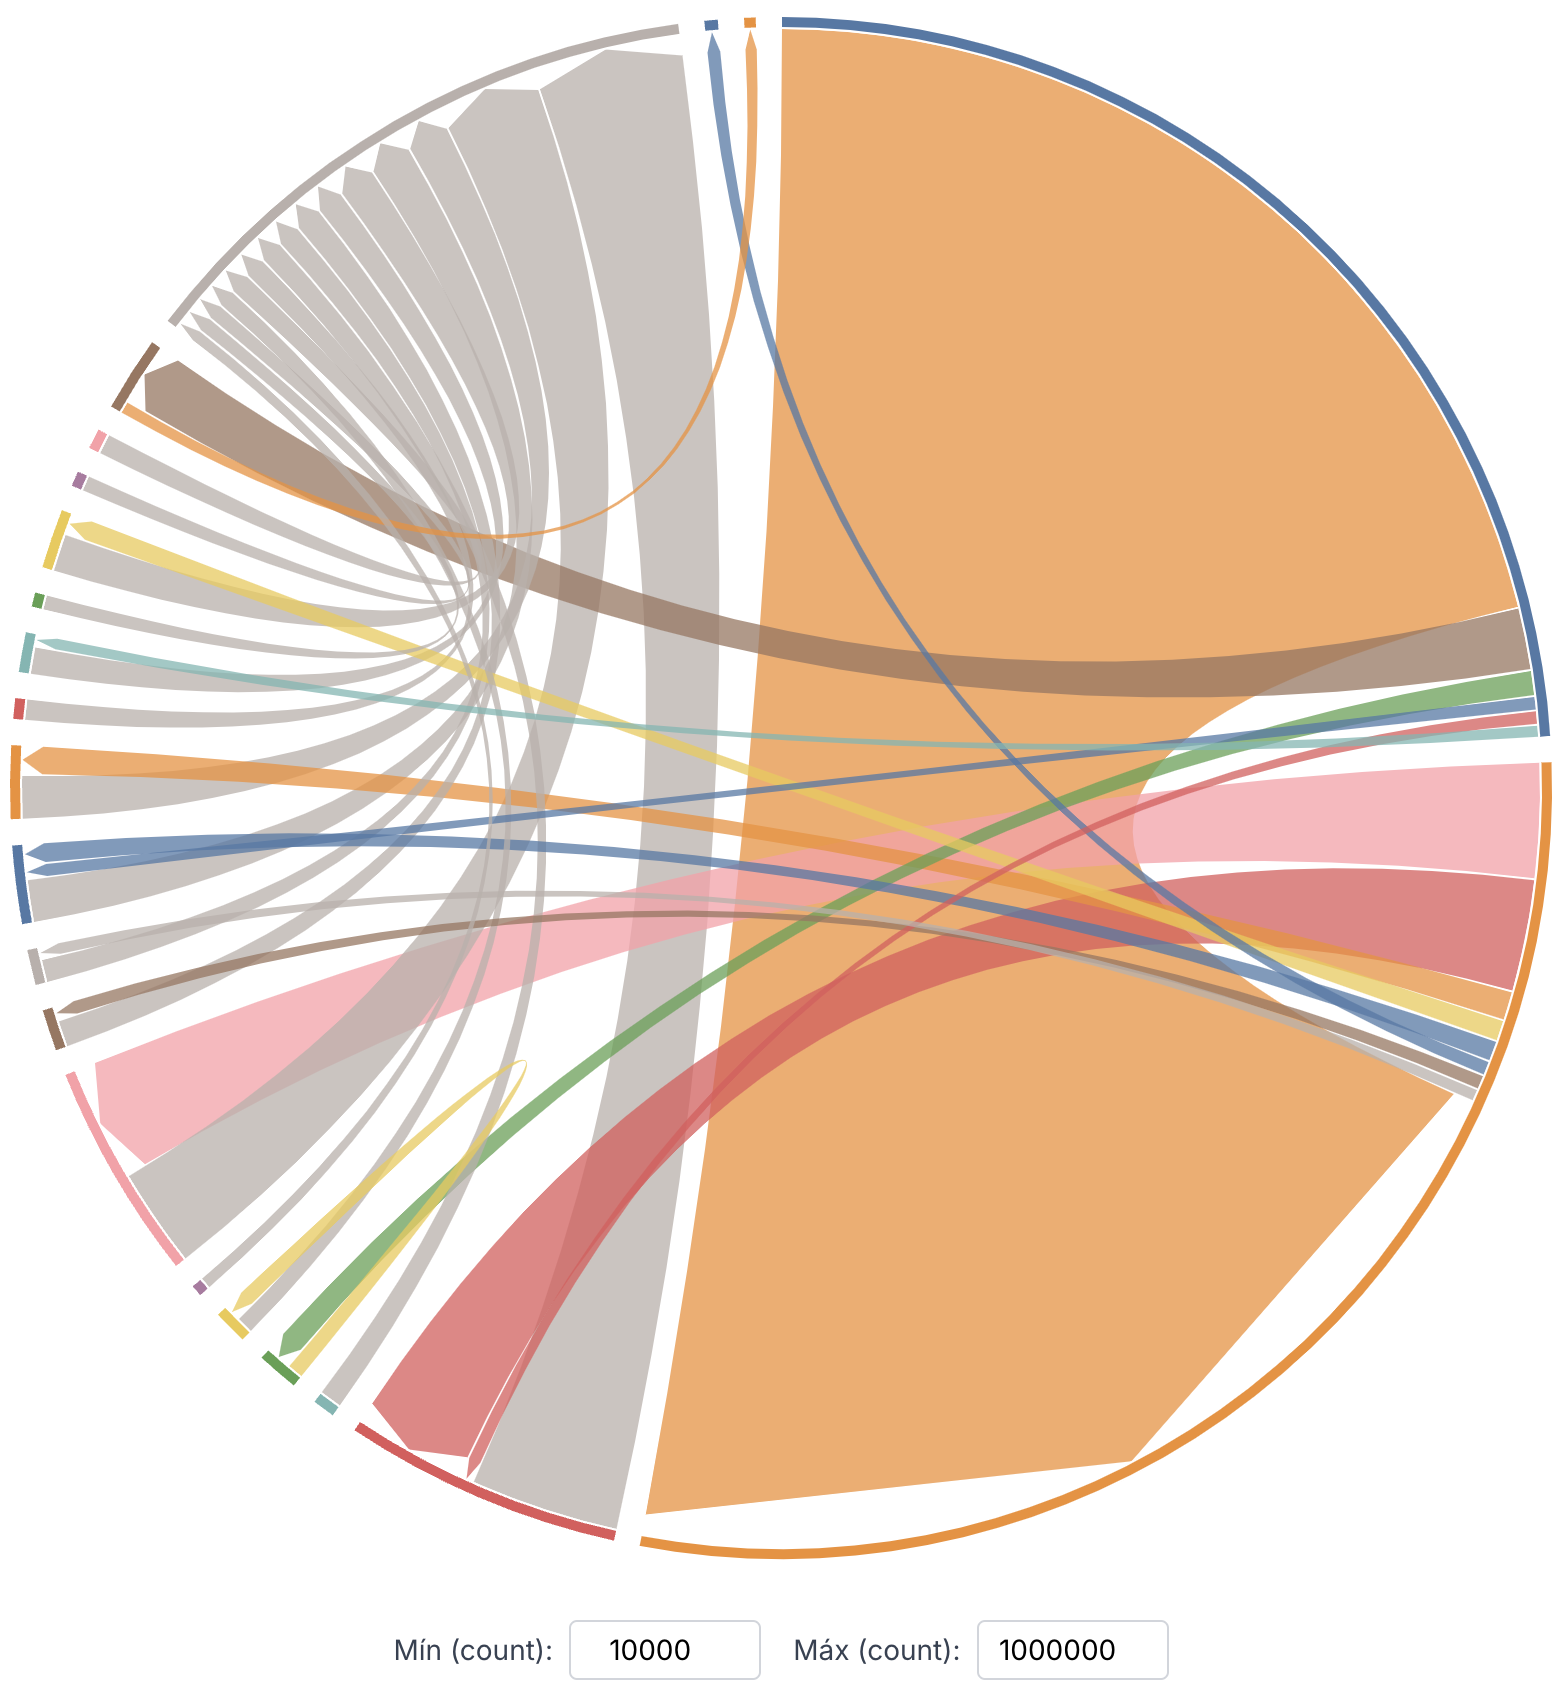
\includegraphics[width=0.88\textwidth]{imagenes/chart-flows.png}}
  \caption{Flujos hospitalarios}
  \label{fig:chart-flows}
\end{figure}


